\documentclass[a4paper,titlepage,oneside,final]{scrreprt} %% Wenn fertig dann draft->final
\usepackage{amsmath}
%\usepackage[latin1]{inputenc}
\usepackage[pdftex]{graphicx}
\usepackage{amsfonts}
\usepackage{txfonts} % F�r Buchstaben aus Def. 2.1 Kyas
%\usepackage{pxfonts}
\usepackage{stmaryrd} % \llparenthesis
\usepackage{amssymb}
\usepackage{hyperref}
\usepackage{color}
\definecolor{darkblue}{rgb}{0,0,.5}
\hypersetup{pdftex=true, colorlinks=true, breaklinks=true, linkcolor=darkblue, menucolor=darkblue, pagecolor=darkblue, urlcolor=darkblue, citecolor=darkblue}
\usepackage{makeidx}
%\usepackage{fancyhdr}
\usepackage{color}
\usepackage{footnpag}
\title{USE \\ A UML based Specification Environment\\{\large \emph{Preliminary Version 0.1}}}
\author{Database Systems Group\\
Bremen University}
%\input{fancyOrNot}
%\input{nochEinFancy}
%\pagestyle{fancy}
\makeindex
\begin{document}
\maketitle
\section*{Version 0.1}
This document represents the first version of the USE documentation.
Several section will be completed, added or changed in the following
versions (e.g. the USE Generator sections).
\newpage
\tableofcontents
\listoffigures
%\listoftables
\chapter{Introduction to USE}
USE is a system for the specification of information systems.
It is based on a subset of the Unified Modeling Language (UML) \cite{uml:00-03-01}.
\section{Overview of USE Features}
A USE specification contains a textual description of a model
using features found in UML class diagrams (classes, associations, etc.).
Expressions written in the Object Constraint Language (OCL) are used to specify
additional integrity constraints on the model. A model can be animated to validate
the specification against non-formal requirements. System states (snapshots of a
running system) can be created and manipulated during an animation. For each
snapshot the OCL constraints are automatically checked. Information about a system
state is given by graphical views. OCL expressions can be entered and evaluated to
query detailed information about a system state.
\section{Working with USE}
This section outlines the general workflow for the specification and validation of a UML model.
Figure \ref{fig:workflow} gives a general view of the USE approach. Within this
section we use an example model specifying the class $\mathit{Car}$ including
an attribute $\mathit{mileage}$ of type $\mathit{Integer}$ and an
operation $\mathit{increaseMileage}$ with one formal parameter an no return value.
\begin{figure}[ht]
\centering
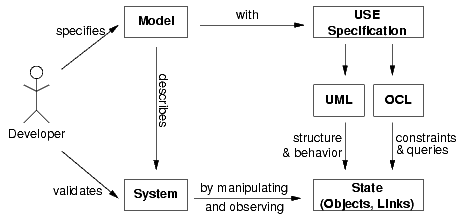
\includegraphics[scale=0.7]{Pictures/workflow.png}
\caption{Overview of the Specification Workflow}
\label{fig:workflow}
\end{figure}
\subsection{Specifying a UML Model}
The USE tool expects a textual description of a model
and its constraints as input. (see section \ref{SpecWithUSE}) The example must therefore be
translated into a USE specification\footnote{A possible extension to
USE would be the import of an XMI file created by a CASE tool like Argo
UML\footnote{http://argouml.tigris.org/} or Rational Rose} by using an external
text editor.
The USE specification of the example model is shown below.
\begin{verbatim}
model Cars

class Car
attributes
  mileage : Integer
operations
  increaseMileage(kilometers : Integer)
end
\end{verbatim}
\subsection{Running USE}
The following command can be used to invoke USE on the example specification.\footnote{Assuming
the current working directory is the top-level directory of the
distribution and the bin directory is added to your PATH environment variable.}
\begin{verbatim}
use ../examples/Documentation/Cars/Cars.use
\end{verbatim}
This command will compile and check the file \verb+Cars.use+.
There are currently two kinds of user interfaces which can be used simultaneously.
The first one is a command line interface where you enter commands at a prompt.
The output should be similar to the following.
\begin{verbatim}
loading properties from: /home/opti/use/etc/use.properties
loading properties from: /home/opti/.userc
use version 2.3.1, Copyright (C) 1999-2006 University of Bremen
compiling specification...
Model Cars (1 class, 0 associations, 0 invariants, 1 operation, 0 pre-/postconditions)
Enter `help' for a list of available commands.
use>
\end{verbatim}
To start USE without loading a specification use the command \verb+use+.
\subsection{USE Shell - The Command Line Interface}
After loading a specification you can enter commands at the prompt.
\footnote{Try 'help' for a list of available commands.} For example,
you can enter OCL expressions by starting the input with a question
mark. The expression will be evaluated and its result will be shown,
e.g.:
\begin{verbatim}
use> ? Set{1,2,3}->select(e | e > 1)
-> Set{2,3} : Set(Integer)
\end{verbatim}
The command line interface is useful for experienced users and for automated validation procedures
since commands can be read from a script file. The graphical user interface is easier
to learn and provides different ways of visualizing a system state.
By default both interfaces are launched. \footnote{Unless you specify the switch -nogui at startup time.}
\subsection{Graphical User Interface}
The window that appears after starting USE can
be seen in the screen shot in figure \ref{fig:StartCars}.
On the left is a tree view showing the contents (classes, associations,
invariants, and pre- and postconditions) of the model.\\
\begin{figure}[ht]
\centering
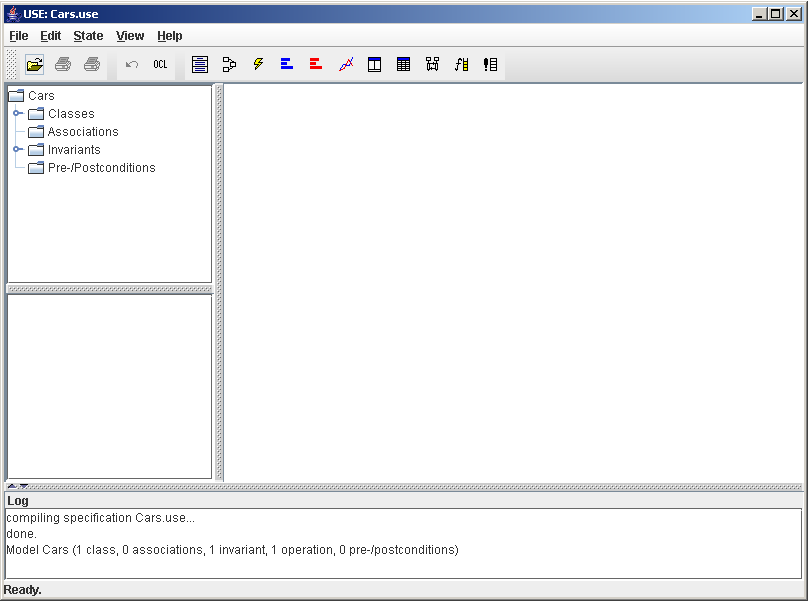
\includegraphics[scale=0.5]{Screenshots/GUI/StartCars.png}
\caption{Graphical User Interface after starting USE with the Cars Example}
\label{fig:StartCars}
\end{figure}\\
The next figure \ref{fig:CarsInv}
shows the expanded tree with all model elements. The invariant
is selected and its definition is shown in the panel below the tree.\\
\begin{figure}[ht]
\centering
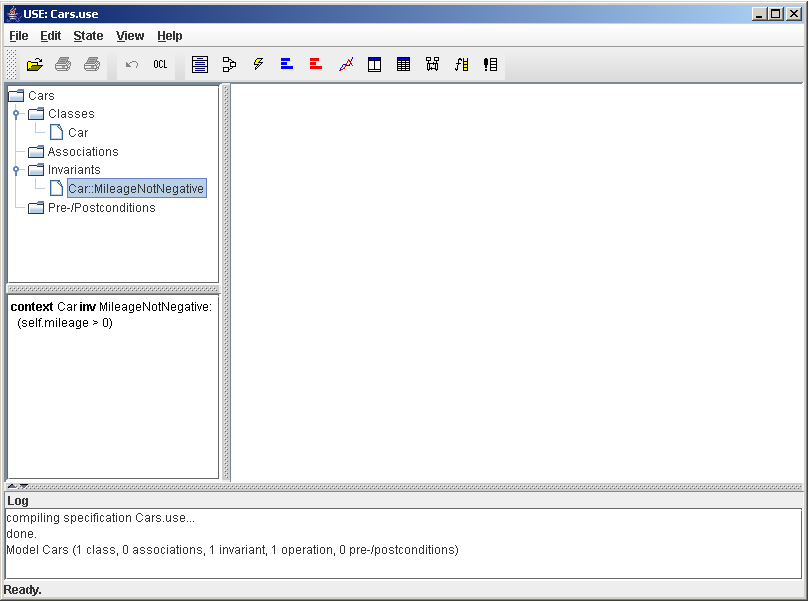
\includegraphics[scale=0.5]{Screenshots/GUI/CarsInv.png}
\caption{Expanded tree with all model elements}
\label{fig:CarsInv}
\end{figure}\\
The large area on the right is a workspace where you can open
views visualizing different aspects of a system. Views can be
created any time by choosing an entry from the view menu or directly
by a toolbar button. There is no limit on active views. The next screenshot shown in
figure \ref{fig:WorkingspaceViews}
displays the main window after the creation of four views.
\begin{figure}[ht]
\centering
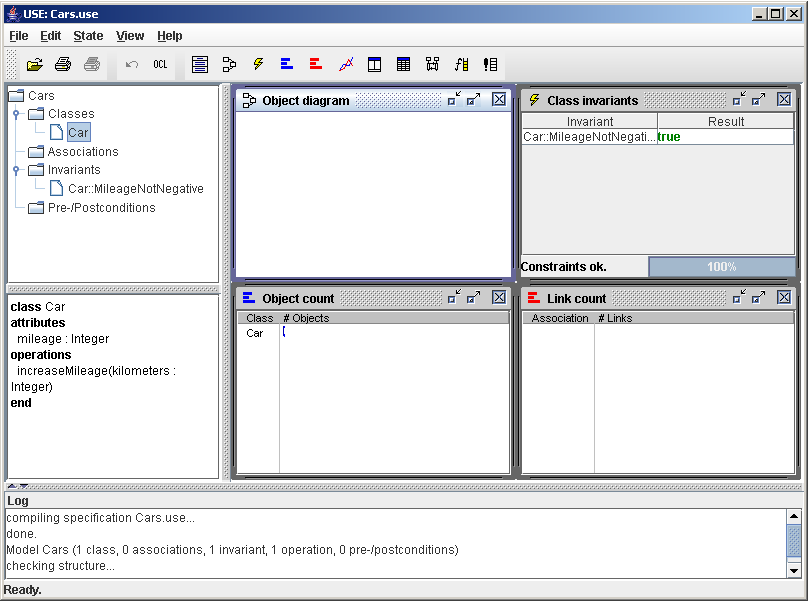
\includegraphics[scale=0.5]{Screenshots/GUI/WorkingspaceViews.png}
\caption{Main window with four different views}
\label{fig:WorkingspaceViews}
\end{figure}
The two lower views list the names of classes and associations defined
in the model and show the number of objects and links in the current system state.
The initial system state is empty, i.e., there are no objects and links yet.
The view at the upper right displays a list of OCL invariants and their results.
As you can see, all invariants are true in the empty system state. Finally, the
upper left view will show an object diagram once we have created objects and links.
\subsection{Creating Objects and Setting Attributes}
Now you can create and destroy objects of type $\mathit{Car}$ and set their attributes.
More complex specifications allow more commands to manipulate the system state. (see
section \ref{ShellCommands}).\\
We create two objects $\mathit{smallCar}$ and $\mathit{bigCar}$ and set their
mileage to $2000$ resp. $-1500$ kilometers. The commands are shown below. They can
be entered step by step or by reading in a command file. To read in the corresponding
command file use the following USE command: \verb+open ../examples/Documentation/Cars/Cars.cmd+
\begin{verbatim}
!create smallCar : Car
!create bigCar : Car

!set smallCar.mileage := 2000
!set bigCar.mileage := -1500
\end{verbatim}
\subsection{Checking OCL Invariants}
After creating the system state the
Class Invariant View shows that $\mathit{MileageNotNegative}$
is violated. (see figure \ref{fig:InvFailed})\\
\begin{figure}[ht]
\centering
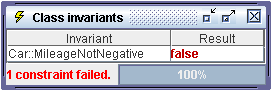
\includegraphics[scale=0.7]{Screenshots/GUI/Views/InvFailed.png}
\caption{Constraint failed}
\label{fig:InvFailed}
\end{figure}\\
To get more information you can double click on the failed invariant.
This opens the Evaluation Browser showing the evaluation of the
marked invariant. In figure \ref{fig:InvFailedBrowser}
you can see, that object $\mathit{bigCar}$ violates the invariant
because its mileage is a negative number.
\begin{figure}[ht]
\centering
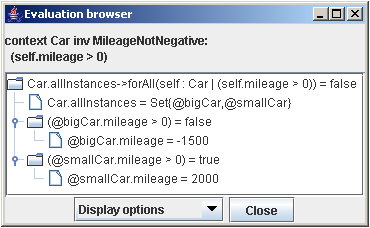
\includegraphics[scale=0.7]{Screenshots/GUI/InvFailedBrowser.png}
\caption{Evaluation of the violated invariant}
\label{fig:InvFailedBrowser}
\end{figure}
\subsection{Evaluating OCL Expressions}
The OCL parser and interpreter of USE allows the evaluation of arbitrary
OCL expressions. The menu item \verb+State|Evaluate OCL expression+
opens a dialog where expressions can be entered and evaluated (see figure \ref{fig:EvalSetExpr}).\\
\begin{figure}[ht]
\centering
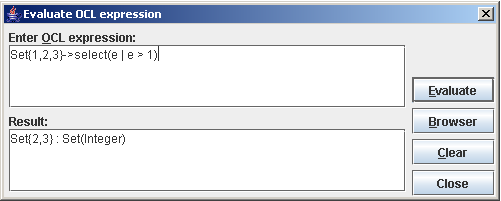
\includegraphics[scale=0.7]{Screenshots/GUI/EvalSetExpr.png}
\caption{Evaluating a simple select expression}
\label{fig:EvalSetExpr}
\end{figure}\\
The example in figure \ref{fig:EvalSelectExpr} shows a more complex expression
with $\mathit{allInstances}$ and the collection operations $\mathit{select}$, $\mathit{collect}$
and $\mathit{exists}$.
\begin{figure}[ht]
\centering
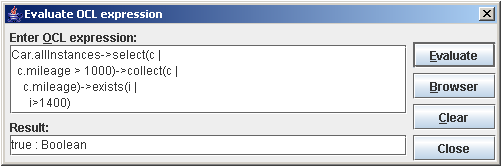
\includegraphics[scale=0.7]{Screenshots/GUI/EvalSelectExpr.png}
\caption{Evaluating a more complex expression}
\label{fig:EvalSelectExpr}
\end{figure}
\section{Formal Background}
The USE specification language is based on UML and OCL.
Due to the semi formal definition of early OCL versions, there were language
constructs whose interpretation was ambiguous or unclear \cite{GogollaRichtersUML:1998}.
In \cite{GogollaRichtersOCL:1998} and \cite{GogollaRichters:1999}
we have presented a formalization of OCL which was designed to provide a solution
for most of the problems and which became part of UML 1.4/1.5. The USE approach to validation
is described in \cite{GogollaRichters:2000} and \cite{richters:phd}. Several other papers of our group employing USE
can be found in the publications of our group.\footnote{http://www.db.informatik.uni-bremen.de/publications/}
\section{Examples inspected within this documentation}\label{examplesDocu}
Beside the cars example there are four examples, which are treated in
the course of this documentation.
\subsection{Employees, Departments and Projects}
This example specifies employees working in at least one department.
They work on an arbitrary number of projects, which are controlled by exactly one
department.\\
Persons, departments and projects have names identifying them. Departments, which have different locations,
and projects have specific budgets. Persons are paid for their job.
They have a regular salary. (see figure \ref{fig:exampleModel})
\begin{figure}[ht]
\centering
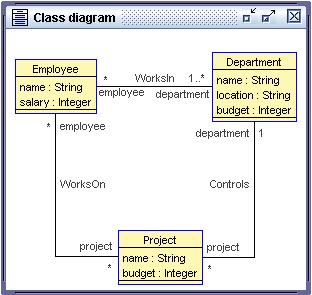
\includegraphics[scale=0.7]{Pictures/cls-EDP.png}
\caption{Class diagram of the Employees, Departments and Projects example}
\label{fig:exampleModel}
\end{figure}
\subsection{Persons and Companies}
The UML class diagram in figure \ref{fig:DiagramPersonCompany}
shows an altered model representing persons and companies.
Persons have a name, an age, and a salary, which can be raised
with the operation $\mathit{raiseSalary}$ by a specific amount.
They work for at most one company, which has a name and a location.
Companies can hire and fire persons.
\begin{figure}[ht]
\centering
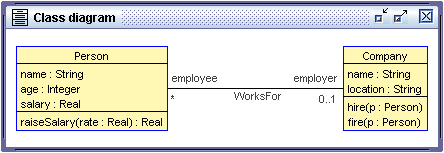
\includegraphics[scale=0.7]{Pictures/cls-Employee.png}
\caption{Class diagram of the Person \& Company example}
\label{fig:DiagramPersonCompany}
\end{figure}
\subsection{Graphs}\label{graphsExample}
This example is modeling a graph structure.
Objects of class $\mathit{Node}$ represent nodes of a graph
that can be connected by edges. Each node can be
connected to an arbitrary number of source and target nodes.
The $\mathit{Node}$ class contains an operation $\mathit{newTarget}$. The purpose of this
operation is to create a new node and to insert a new edge
between the source node and the new target node.
\begin{figure}[ht]
\centering
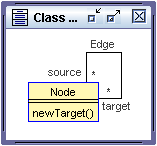
\includegraphics[scale=0.7]{Pictures/GraphClassDiagram.png}
\caption{Class diagram of the Graph example}
\label{fig:GraphClassDiagram}
\end{figure}
\subsection{Factorial}\label{factorialExample}
The factorial example shows how operation calls may be nested in the simulation.
It also shows that postconditions may be specified on operations
without side effects. An OCL expression can be given to describe
the computation of a side effect free operation. In the example,
we use a recursive definition of the factorial function.
There is only one class $\mathit{Rec}$.
\begin{figure}[ht]
\centering
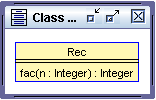
\includegraphics[scale=0.7]{Pictures/NestedClassDiagram.png}
\caption{Class diagram of factorial example}
\label{fig:FactorialClassDiagram}
\end{figure}
\chapter{Specifying a UML Model with USE}\label{SpecWithUSE}
To define a USE specifications you need an external text editor.
The syntactic elements are clarified by a grammar defined with the Extended Backus-Naur Form.
\section{Defining a UML Model}
Every UML Model \index{UML Model} has a name and an optional body.
\begin{description}
\item[Syntax:]
\begin{eqnarray*}
\langle\mathit{umlmodel\rangle}&\Coloneqq& \verb+model+ ~
\langle\mathit{modelname}\rangle~ [~\langle\mathit{modelbody}\rangle~]\\
\langle\mathit{modelname}\rangle &\Coloneqq& \langle\mathit{name}\rangle
\end{eqnarray*}
\item[Example:] The models name is \verb+Fruits+.
\begin{verbatim}
model Fruits
...
\end{verbatim}
\end{description}
The model body\index{UML Model!Body} consists of at least one class definition
and an arbitrary number of association definitions.
Enumeration definitions are allowed at the top of the body.
At the end of the specification OCL constraints may be defined.
\begin{description}
\item[Syntax:]
\begin{eqnarray*}
\langle\mathit{modelbody}\rangle &\Coloneqq&
\{~\langle\mathit{enumerationdefinition}\rangle~\}\\
&&\{~\langle\mathit{associationdefinition}\rangle~|~
\langle\mathit{associationclassdefinition}\rangle~\}\\
&&\langle\mathit{classdefinition}\rangle\\
&&\{~\langle\mathit{classdefinition}\rangle ~|~
\langle\mathit{associationdefinition}\rangle~
|~\langle\mathit{associationclassdefinition}\rangle~\}\\
&&[~\verb+constraints+ ~\{~\langle\mathit{constraintdefinition}\rangle~\}~]
\end{eqnarray*}
\end{description}
\section{Specification Elements}
The following sections describe all available elements, which can be used
in the model body.
\subsection{Enumerations}
Enumerations \index{UML Model!Enumeration} may be added at the top of
the model body.
\begin{description}
\item[Syntax:]
\begin{eqnarray*}
\langle\mathit{enumerationdefinition}\rangle &\Coloneqq&
\verb+enum+~\langle\mathit{enumerationname}\rangle~\verb+{+~
\langle\mathit{elementname}\rangle~\{~\verb+,+~\langle\mathit{elementname}\rangle~\}~\verb+}+\\
\langle\mathit{enumerationname}\rangle &\Coloneqq&
\langle\mathit{name}\rangle\\
\langle\mathit{elementname}\rangle &\Coloneqq&
\langle\mathit{name}\rangle
\end{eqnarray*}
\item[Example:] An enumeration definition with three elements.
\begin{verbatim}
enum Flatware {Spoon, Fork, Knife}
\end{verbatim}
\end{description}
\subsection{Classes}
A class \index{UML Model!Class} has a name and optionally attribute and operation definitions.
It may be defined as an abstract class.
\begin{description}
\item[Syntax:]
\begin{eqnarray*}
\langle\mathit{classdefinition}\rangle &\Coloneqq& [~\verb+abstract+~]~\verb+class+~
\langle\mathit{classname}\rangle~[~\verb+<+~\langle\mathit{classname}\rangle~
\{~\verb+,+~\langle\mathit{classname}\rangle~\}~]\\
&&[~\verb+attributes+~\{~\langle\mathit{attributename}\rangle
~\verb+:+~\langle\mathit{type}\rangle~\}~]\\
&&[~\verb+operations+~\{~\langle\mathit{operationdeclaration}\rangle
~[~\verb+=+~\langle\mathit{oclexpression}\rangle~]\\
&&\{~\langle\mathit{preconditiondefinition}\rangle~|~
\langle\mathit{postconditiondefinition}\rangle~\}~\}~]\\
&& [~\verb+constraints+~\{~\langle\mathit{invariantdefinition}\rangle~\}~]\\
&& \verb+end+\\
\langle\mathit{classname}\rangle &\Coloneqq& \langle\mathit{name}\rangle\\
\langle\mathit{attributename}\rangle &\Coloneqq& \langle\mathit{name}\rangle
\end{eqnarray*}
\item[Example:] The example shows five different class definitions.
The class $\mathit{Apple}$ inherits two and the class
$\mathit{Banana}$ one class.
The class $\mathit{Lemon}$ is abstract and class $\mathit{Banana}$ defines pre- and postconditions
for the operation $\mathit{peel}$ within its body.
The class $\mathit{Peach}$ shows how invariants can be integrated
into the classes body.
\begin{verbatim}
class Apple < Orange, Lemon
end

abstract class Orange
attributes
  juice : Boolean
end

class Lemon
operations
  squeeze(i : Integer) : Integer = i + 1
end

class Banana < Lemon
attributes
  flatware : Set(Sequence(Flatware))
operations
  peel() : String = 'abcd'
      pre: true
      post: 2 = 2
      post: result = 'theResult'
end

class Peach
attributes
operations
constraints
  inv: 3 > 2
  inv neverViolated: true
end
\end{verbatim}
\end{description}
\subsection{Associations}
It is possible to define n ary associations \index{UML Model!Association}. The definition requires a name,
at least two participating classes and multiplicity information. Role names are optional.
\begin{description}
\item[Syntax:]
\begin{eqnarray*}
\langle\mathit{associationdefinition}\rangle &\Coloneqq&
(~\verb+association+~|~\verb+composition+~|~\verb+aggregation+~)\\
&&\langle\mathit{associationname}\rangle~\verb+between+\\
&&\langle\mathit{classname}\rangle~\verb+[+~\langle\mathit{multiplicity}\rangle~
\verb+]+~[~\verb+role+~\langle\mathit{rolename}\rangle~]~[~\verb+ordered+~]\\
&&\langle\mathit{classname}\rangle~\verb+[+~\langle\mathit{multiplicity}\rangle~
\verb+]+~[~\verb+role+~\langle\mathit{rolename}\rangle~]~[~\verb+ordered+~]\\
&&\{~\langle\mathit{classname}\rangle~\verb+[+~\langle\mathit{multiplicity}\rangle~
\verb+]+~[~\verb+role+~\langle\mathit{rolename}\rangle~]~[~\verb+ordered+~]~\}\\
&&\verb+end+\\
\langle\mathit{multiplicity}\rangle &\Coloneqq&
(~\verb+*+~|~\langle\mathit{digit}\rangle~\{~\langle\mathit{digit}\rangle~\}~
[~\verb+..+~(~\verb+*+~|~\langle\mathit{digit}\rangle~\{~\langle\mathit{digit}\rangle~\}~)~]~)\\
&& \{~\verb+,+~(~\verb+*+~|~\langle\mathit{digit}\rangle~\{~\langle\mathit{digit}\rangle~\}~
[~\verb+..+~(~\verb+*+~|~\langle\mathit{digit}\rangle~\{~\langle\mathit{digit}\rangle~\}~)~]~)~\}\\
\langle\mathit{associationname}\rangle &\Coloneqq& \langle\mathit{name}\rangle\\
\langle\mathit{rolename}\rangle &\Coloneqq& \langle\mathit{name}\rangle
\end{eqnarray*}
\item[Example:] This Examples shows a binary and a tertiary association with different
multiplicities and optional role names. The first association is defined as
a composition. The diamond appears at the first participating class.
You may order the elements by using
the keyword \verb+ordered+.
\begin{verbatim}
composition AppleSpritzer between
  Apple[*] role base
  Lemon[1..8,10,15..*] role flavor
end

association Ingredients between
  Apple[*] role mainIngredient
  Orange[1]
  Lemon[1..*] role lemon ordered
end
\end{verbatim}
\end{description}
\subsection{Association classes}
Association classes \index{UML Model!Associationclass} combine the body elements of classes and associations.
\begin{description}
\item[Syntax:]
\begin{eqnarray*}
\langle\mathit{associationclassdefinition}\rangle &\Coloneqq&
[~\verb+abstract+~]~\verb+associationclass+~
\langle\mathit{classname}\rangle\\
&&[~\verb+<+~\langle\mathit{classname}\rangle~
\{~\verb+,+~\langle\mathit{classname}\rangle~\}~]~\verb+between+\\
&&\langle\mathit{classname}\rangle~\verb+[+~\langle\mathit{multiplicity}\rangle~
\verb+]+~[~\verb+role+~\langle\mathit{rolename}\rangle~]~[~\verb+ordered+~]\\
&&\langle\mathit{classname}\rangle~\verb+[+~\langle\mathit{multiplicity}\rangle~
\verb+]+~[~\verb+role+~\langle\mathit{rolename}\rangle~]~[~\verb+ordered+~]\\
&&\{~\langle\mathit{classname}\rangle~\verb+[+~\langle\mathit{multiplicity}\rangle~
\verb+]+~[~\verb+role+~\langle\mathit{rolename}\rangle~]~[~\verb+ordered+~]~\}\\
&&[~\verb+attributes+~\{~\langle\mathit{attributename}\rangle
~\verb+:+~\langle\mathit{type}\rangle~\}~]\\
&&[~\verb+operations+~\{~\langle\mathit{operationdeclaration}\rangle
~[~\verb+=+~\langle\mathit{oclexpression}\rangle~]\\
&&\{~\langle\mathit{preconditiondefinition}\rangle~|~
\langle\mathit{postconditiondefinition}\rangle~\}~\}~]\\
&& [~\verb+constraints+~\{~\langle\mathit{invariantdefinition}\rangle~\}~]\\
&& \verb+end+
\end{eqnarray*}
\item[Example:] The example defines an association class between
two classes. It has two attributes and one operation, which is no
query.
\begin{verbatim}
associationclass FruitSalad < Orange
 between
  Banana[0..1]
  Apple[1..*]
attributes
  name : String
  weight : Real
operations
  putIn(apple : Apple, banana : Banana)
end
\end{verbatim}
\end{description}
\subsection{Constraints}
The keyword \verb+constraints+ \index{UML Model!Constraint} indicates the begin of constraint definition segment.
An arbitrary number of invariants may be defined in context of a class.
In addition to that, you may define pre- and postconditions
to constrain operations. Every constraint can be named.
\begin{description}
\item[Syntax:]
\begin{eqnarray*}
\langle\mathit{constraintdefinition}\rangle &\Coloneqq&
\langle\mathit{invariantcontext}\rangle~|~\langle\mathit{operationcontext}\rangle\\
\langle\mathit{invariantcontext}\rangle &\Coloneqq&
\verb+context+~[~\langle\mathit{variablename}\rangle~\verb+:+~]~\langle\mathit{classname}\rangle\\
&&\{~\langle\mathit{invariantdefinition}\rangle~\}\\
\langle\mathit{operationcontext}\rangle &\Coloneqq&
\verb+context+~\langle\mathit{classname}\rangle~\langle\mathit{operationconstraints}\rangle\\
\langle\mathit{invariantdefinition}\rangle &\Coloneqq&
\verb+inv+~[~\langle\mathit{invariantname}\rangle~]~\verb+:+~\langle\mathit{booleanoclexpression}\rangle\\
\langle\mathit{operationconstraints}\rangle &\Coloneqq&
\verb+::+~\langle\mathit{operationdeclaration}\rangle\\
&&(~\langle\mathit{preconditiondefinition}\rangle~|~\langle\mathit{postconditiondefinition}\rangle~)\\
&&\{~\langle\mathit{preconditiondefinition}\rangle~|~
\langle\mathit{postconditiondefinition}\rangle~\}\\
\langle\mathit{preconditiondefinition}\rangle &\Coloneqq&
\verb+pre+~[~\langle\mathit{preconditionname}\rangle~]~
\verb+:+~\langle\mathit{booleanoclexpression}\rangle\\
\langle\mathit{postconditiondefinition}\rangle &\Coloneqq&
\verb+post+~[~\langle\mathit{postconditionname}\rangle~]~
\verb+:+~\langle\mathit{booleanoclexpression}\rangle~)\\
\langle\mathit{invariantname}\rangle &\Coloneqq& \langle\mathit{name}\rangle\\
\langle\mathit{variablename}\rangle &\Coloneqq& \langle\mathit{name}\rangle\\
\langle\mathit{preconditionname}\rangle &\Coloneqq& \langle\mathit{name}\rangle\\
\langle\mathit{postconditionname}\rangle &\Coloneqq& \langle\mathit{name}\rangle
\end{eqnarray*}
\item[Example:] The first two definitions are showing three invariants of the class $\mathit{Orange}$.
The second definition defines the variable $\mathit{orange}$ which
may be used in the OCL expression similar to $\mathit{self}$. The third invariant is not named. USE
will assign a name like $\mathit{inv2}$ to it.
Two preconditions and one postcondition constrain the Operation $\mathit{squeeze}$ in class
$\mathit{Lemon}$.
\begin{verbatim}
context Orange
 inv OrangeInv: 1 = 1

context orange : Orange
 inv alwaysTrue: orange = orange
 inv: juice = true

context Lemon :: squeeze(i : Integer) : Integer
  pre: i>0
  pre lessThanTenOranges: i<10
  post alwaysTrue: true
\end{verbatim}
\end{description}
\subsection{Operation declarations}
The declaration of an operation \index{UML Model!Operation} consists of the operation name, optional parameters
and the return type.
\begin{description}
\item[Syntax:]
\begin{eqnarray*}
\langle\mathit{operationdeclaration}\rangle &\Coloneqq&
\langle\mathit{operationname}\rangle~\verb+(+~[~\langle\mathit{parameters}\rangle~]~
\verb+)+~[~\verb+:+~\langle\mathit{type}\rangle~]\\
\langle\mathit{parameters}\rangle &\Coloneqq&
\langle\mathit{parametername}\rangle~\verb+:+~\langle\mathit{type}\rangle~
\{~\verb+,+~\langle\mathit{parametername}\rangle~\verb+:+~\langle\mathit{type}\rangle~\}\\
\langle\mathit{operationname}\rangle &\Coloneqq& \langle\mathit{name}\rangle\\
\langle\mathit{parametername}\rangle &\Coloneqq& \langle\mathit{name}\rangle
\end{eqnarray*}
\item[Example:] Three operation declarations are shown within the class definition example.
\end{description}
\subsection{Types}
Types \index{UML Model!Types} may be simple ($\langle\mathit{simpletype}\rangle$) or complex
($\langle\mathit{collectiontype}\rangle$).
\begin{description}
\item[Syntax:]
\begin{eqnarray*}
\langle\mathit{type}\rangle &\Coloneqq& \langle\mathit{collectiontype}\rangle~
|~\langle\mathit{simpletype}\rangle~|~\langle\mathit{enumerationname}\rangle\\
\langle\mathit{collectiontype}\rangle &\Coloneqq& (~\verb+Set+~|~\verb+Bag+~|~\verb+Sequence+~)~
\verb+(+\\
&&\{~\langle\mathit{collectiontype}\rangle~
|~\langle\mathit{simpletype}\rangle~|~\langle\mathit{enumerationname}\rangle~\}~\verb+)+\\
\langle\mathit{simpletype}\rangle &\Coloneqq& \verb+Integer+~|~\verb+Real+~|~\verb+Boolean+~|~
\verb+String+~|~\langle\mathit{classname}\rangle
\end{eqnarray*}
\item[Example:] The attribute $\mathit{flatware}$ has a complex type.
\end{description}
\subsection{Names, Numbers and OCL-Expressions}
\begin{eqnarray*}
\langle\mathit{name}\rangle &\Coloneqq& (~\langle\mathit{letter}\rangle ~|~ \_~)~
\{~\langle\mathit{letter}\rangle~ |~ \langle\mathit{digit}\rangle ~|~ \_~\}\\
\langle\mathit{letter}\rangle &\Coloneqq&  \verb+a+~ |~ \verb+b+~
|~ \dots~ |~ \verb+z+~ | ~\verb+A+~ |~ \verb+B+~ |~ \dots~ | ~\verb+Z+\\
\langle\mathit{digit}\rangle &\Coloneqq& \verb+0+~ |~ \verb+1+~ |~ \dots~ |~ \verb+9+\\
\langle\mathit{oclexpression}\rangle &\Coloneqq&
(^*~\mathrm{Replace~this ~symbol~ by~ an ~ordinary ~OCL ~expression.}~^*)\\
\langle\mathit{booleanoclexpression}\rangle &\Coloneqq&
(^*~\mathrm{Replace~ this ~symbol~ by~ an~ ordinary~ OCL expression}\\
&&\mathrm{which~results ~in~ a ~boolean~ value.}~^*)
\end{eqnarray*}
\section{Specifications of the Examples}
The USE specification of the example models shown in section \ref{examplesDocu} are presented
in this section.
\subsection{Employees, Departments and Projects}\label{EDPspec}
The first part of the specification
shown below describes the structural information of the class diagram.
There are classes with attributes and associations with different multiplicities.
\begin{verbatim}
model Company

-- classes

class Employee
attributes
  name : String
  salary : Integer
end

class Department
attributes
  name : String
  location : String
  budget : Integer
end

class Project
attributes
  name : String
  budget : Integer
end

-- associations

association WorksIn between
  Employee[*]
  Department[1..*]
end

association WorksOn between
  Employee[*]
  Project[*]
end

association Controls between
  Department[1]
  Project[*]
end
\end{verbatim}
We extend the model by the following four constraints which place further restrictions
on systems conforming to the model. The constraints are first given in natural language
and will later be expressed more formally in OCL (Object Constraint Language).
Constraints:
\begin{description}
\item[1.] The number of employees working in a department must be greater or equal
to the number of projects controlled by the department.
\item[2.] Employees get a higher salary when they work on more projects.
\item[3.] The budget of a project must not exceed the budget of the controlling department.
\item[4.] Employees working on a project must also work in the controlling department.
\end{description}
The goal of applying the USE tool is to interactively validate the above model
and the constraints. Objects and links can be created which constitute a system state
reflecting a snapshot of a running system. In every system state,
the constraints are automatically checked for validity.\\\\
In the second part of the specification, we define the constraints in OCL.
Each constraint is defined as an invariant in context of a class.
\begin{verbatim}
-- OCL constraints

constraints

context Department
    -- the number of employees working in a department must
    -- be greater or equal to the number of projects
    -- controlled by the department
  inv MoreEmployeesThanProjects:
    self.employee->size >= self.project->size

context Employee
    -- employees get a higher salary when they work on
    -- more projects
  inv MoreProjectsHigherSalary:
    Employee.allInstances->forAll(e1, e2 |
      e1.project->size > e2.project->size
        implies e1.salary > e2.salary)

context Project
    -- the budget of a project must not exceed the
    -- budget of the controlling department
  inv BudgetWithinDepartmentBudget:
    self.budget <= self.department.budget

    -- employees working on a project must also work in the
    -- controlling department
  inv EmployeesInControllingDepartment:
    self.department.employee->includesAll(self.employee)
\end{verbatim}
The complete specification is also available in the file Demo.use\footnote{http://www.db.informatik.uni-bremen.de/projects/USE/Demo.use}
in the example directory of the distribution.
\subsection{Persons and Companies}\label{personCompanySpec}
Here is the USE specification of the class diagram shown in figure \ref{fig:DiagramPersonCompany}.
\begin{verbatim}
model Employee

-- classes

class Person
attributes
  name : String
  age : Integer
  salary : Real
operations
  raiseSalary(rate : Real) : Real
end

class Company
attributes
  name : String
  location : String
operations
  hire(p : Person)
  fire(p : Person)
end

-- associations

association WorksFor between
  Person[*] role employee
  Company[0..1] role employer
end
\end{verbatim}
We add pre- and postconditions for the $\mathit{hire}$ and $\mathit{fire}$ operations
in class Company. The USE specification is extended as follows.
\begin{verbatim}
-- constraints

constraints

context Company::hire(p : Person)
  pre  hirePre1: p.isDefined()
  pre  hirePre2: employee->excludes(p)
  post hirePost: employee->includes(p)

context Company::fire(p : Person)
  pre  firePre:  employee->includes(p)
  post firePost: employee->excludes(p)
\end{verbatim}
The first precondition of the hire operation is named $\mathit{hirePre1}$ and makes sure
that the operation can only be called with a well defined person object.\footnote{Note that the
operation $\mathit{isDefined}$ is a USE extension. It is not possible
to express this constraint with standard OCL.} The second precondition $\mathit{hirePre2}$
makes sure that the person passed as parameter $p$ is not already an employee of
the company. The postcondition $\mathit{hirePost}$ guarantees that after the operation
has exited, the person actually has been added to the set of employees.
The constraints for the operation $\mathit{fire}$ work just the other way round.
\subsection{Graphs}\label{graphsSpec}
The USE specification of the graphs example (\ref{graphsExample}) is shown below.
\begin{verbatim}
model Graph

class Node
operations
  newTarget()
end

association Edge between
  Node[*] role source
  Node[*] role target
end

constraints

context Node::newTarget()
  -- the operation must link exactly one target node
  post oneNewTarget:
    (target - target@pre)->size() = 1

  -- the target node must not exist before
  post targetNodeIsNew:
    (target - target@pre)->forAll(n | n.oclIsNew())
\end{verbatim}
The postcondition $\mathit{targetNodeIsNew}$ also demonstrates the
application of the OCL operation $\mathit{oclIsNew}$ to check for
the creation of new objects.
\subsection{Factorial}\label{factorialSpec}
The factorial example presented in section \ref{factorialExample} is specified below.
\begin{verbatim}
model NestedOperationCalls

class Rec
operations
  fac(n : Integer) : Integer =
    if n <= 1 then 1 else n * self.fac(n - 1) endif
  end

constraints

context Rec::fac(n : Integer) : Integer
  pre:  n > 0
  post: result = n * fac(n - 1)
\end{verbatim}
The postcondition reflects the inductive case of the definition
of the factorial function.
\chapter{Analyzing the formal Specification}
After specifying a UML model within a \verb+.use+ file
you can open it with USE. The USE system will parse and type check the file
automatically. Possible errors are listed in the log window. (see section \ref{logWindow})
\section{Creating System States}
The Employees, Departments and Projects example specified in section \ref{EDPspec}
is used to show how system states can be created and invariants evaluated.\\\\
Objects can be created by selecting a class and specifying a name for the object.
The menu command \verb+State|Create object+ opens a dialog where this information can be entered
(shown in figure \ref{fig:CreateObject}).
\begin{figure}[ht]
\centering
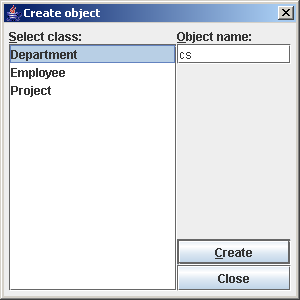
\includegraphics[scale=0.7]{Screenshots/GUI/CreateObject.png}
\caption{Create object dialog}
\label{fig:CreateObject}
\end{figure}\\
Alternatively, the following command can be used at the shell to achieve the same effect.
\begin{verbatim}
use> !create cs:Department
\end{verbatim}
And, even simpler, an object can be created via drag \& drop.
Just select a class in the model browser (see section \ref{low})
and drag it to the object diagram.\\\\
Figure \ref{fig:ViewsWithObject} is similar to figure \ref{fig:WorkingspaceViews},
but the specification changed to the Employees, Departments and Projects example
and the object $\mathit{cs}$ was created.
The lower left view indicates that
there is now one $\mathit{Department}$ object,
and the object diagram shows this object graphically.\\
\begin{figure}[ht]
\centering
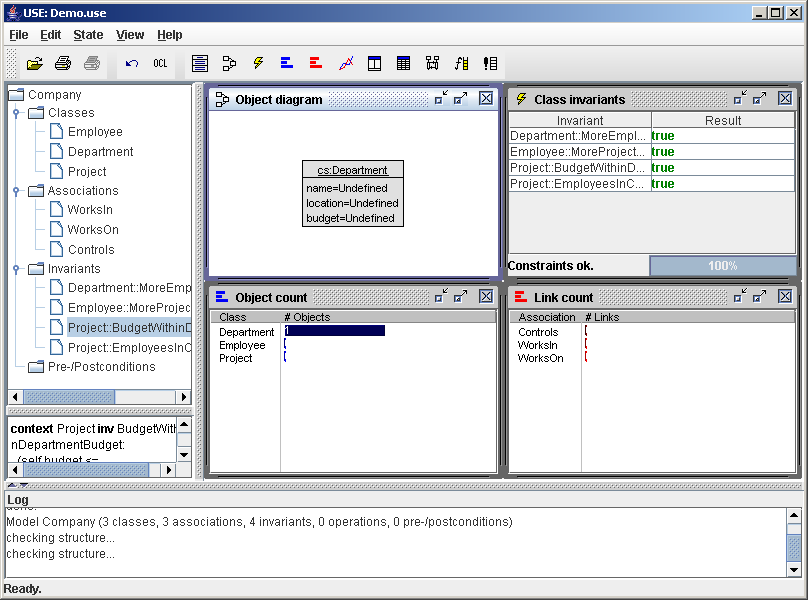
\includegraphics[scale=0.5]{Screenshots/GUI/ViewsWithObject.png}
\caption{Main window with views after creating a new object}
\label{fig:ViewsWithObject}
\end{figure}\\
A context menu available on a right mouse click in the object
diagram provides several display options. For example, the automatic
layout can be turned off, the layout of the diagram can be saved and
restored from a file, etc. In the previous picture we have turned on
the display of attribute values. You can see that the attribute values
of the $\mathit{Department}$ object are all undefined.
For changing attribute values, we can use the \verb+set+ command:
\begin{verbatim}
use> !set cs.name := 'Computer Science'
use> !set cs.location := 'Bremen'
use> !set cs.budget := 10000
\end{verbatim}
Attributes can also be changed with an Object Properties View.
If you choose \verb+View|Create|+ \verb+Object Properties+ from the \verb+View+ menu
and select the $\mathit{cs}$ object, you get the view shown
in figure \ref{fig:ObjectProperties}
where you can inspect and change attributes of the selected object.\\
\begin{figure}[ht]
\centering
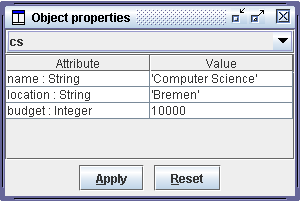
\includegraphics[scale=0.7]{Screenshots/GUI/ObjectProperties.png}
\caption{Object Properties View}
\label{fig:ObjectProperties}
\end{figure}\\
We continue by adding two $\mathit{Employee}$ objects and setting their attributes.\footnote{Again,
we use the command line interface here, but the same can be
achieved by using the previously discussed steps in the graphical user interface.}
\begin{verbatim}
use> !create john : Employee
use> !set john.name := 'John'
use> !set john.salary := 4000
use> !create frank : Employee
use> !set frank.name := 'Frank'
use> !set frank.salary := 4500
\end{verbatim}
Now we have three objects, a department and two employees,
but still no connections between them. The layout in the object
diagram is continuously refined and updated. This can be turned off
by deselecting the option \verb+Auto-Layout+ in the context menu of the object diagram.\\\\
The previous commands resulted in an invalid system state.
This is discussed in detail in the next section.
\subsection{Model Inherent Constraints}\label{modelinherent}
The invariant view indicates some problem with the new system state.
The message says: \verb+Model inherent constraints violated+. Model inherent
constraints are constraints defined implicitly by a UML model (in contrast
to explicit OCL constraints). The details about this message are shown in the log
panel at the bottom of the screen. (see figure \ref{fig:LogWindow})
They are also available by issuing a check command at the prompt:
\begin{verbatim}
use> check
checking structure...
Multiplicity constraint violation in association `WorksIn':
  Object `frank' of class `Employee' is connected to 0 objects of
    class `Department' via role `department'
  but the multiplicity is specified as `1..*'.
Multiplicity constraint violation in association `WorksIn':
  Object `john' of class `Employee' is connected to 0 objects of
    class `Department' via role `department'
  but the multiplicity is specified as `1..*'.
...
\end{verbatim}
The problem here is that we have specified in the model
that each employee has to be related to at least one department
object. (see the class diagram shown in figure \ref{fig:exampleModel})
In our current state, no employee
has a link to a department. In order to fix this, we insert the missing
links into the $\mathit{WorksIn}$ association:
\begin{verbatim}
use> !insert (john,cs) into WorksIn
use> !insert (frank,cs) into WorksIn
\end{verbatim}
Links can also be inserted by selecting the objects to
be connected in the object diagram and choosing the \verb+insert+ command from the context menu.\\\\
The new state shows the links in the object diagram as red
edges between the $\mathit{Employee}$ objects and the $\mathit{Department}$ object.
(see figure \ref{fig:ViewsWithLinks})
\begin{figure}[ht]
\centering
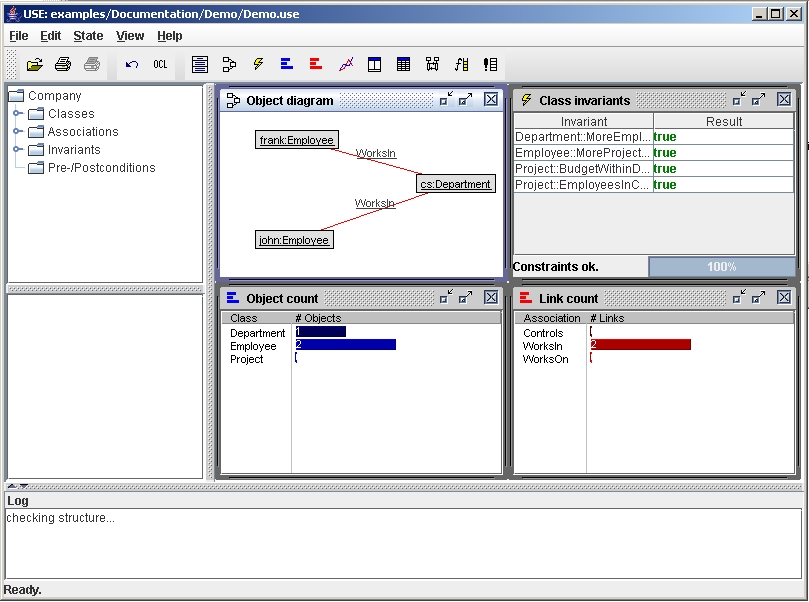
\includegraphics[scale=0.5]{Screenshots/GUI/ViewsWithLinks.png}
\caption{Main window after creating the objects and inserting the links}
\label{fig:ViewsWithLinks}
\end{figure}
\section{Validating Invariants}
We have seen that class invariants are checked automatically
each time a system state changes. This section shows how invariants can
be analyzed. We continue the example by adding two projects and
linking them to the existing employees and the department.
\begin{verbatim}
use> !create research : Project
use> !set research.name := 'Research'
use> !set research.budget := 12000
use>
use> !create teaching : Project
use> !set teaching.name := 'Validating UML'
use> !set teaching.budget := 3000
use>
use> !insert (cs,research) into Controls
use> !insert (cs,teaching) into Controls
use>
use> !insert (frank,research) into WorksOn
use> !insert (frank,teaching) into WorksOn
use> !insert (john,research) into WorksOn
\end{verbatim}
The resulting state is shown in figure \ref{fig:ViewsDemo}.
\begin{figure}[ht]
\centering
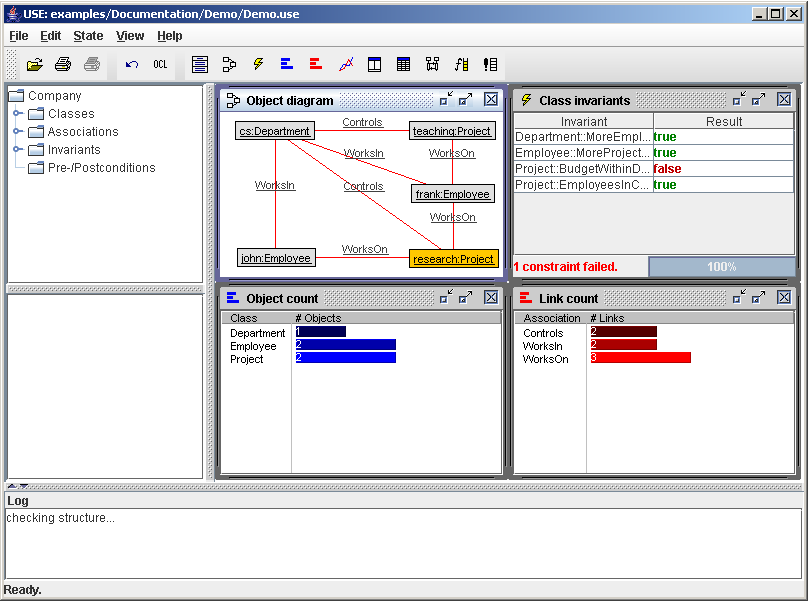
\includegraphics[scale=0.5]{Screenshots/GUI/ViewsDemo.png}
\caption{Main window after reading in the whole Demo.cmd file}
\label{fig:ViewsDemo}
\end{figure}
In this state, three of the four invariants
are true but one fails. The failing one has
the name $\mathit{BudgetWithinDepartmentBudget}$. This invariant states that
the budget of a project must not exceed the budget of the controlling department.
Obviously, one of the two projects in our example must
have a budget higher than the budget of the department.\\
The value $\mathit{false}$ finally resulting from an evaluation of an
invariant is not very helpful in finding the reason for an illegal
system state. An Evaluation Browser provides a more detailed view of
an expression by showing the results of all sub expressions. (see section \ref{evaluationBrowserSec})
Double clicking
on an invariant will open an Evaluation Browser (see figure \ref{fig:EvalBrowserDemo}).
\begin{figure}[ht]
\centering
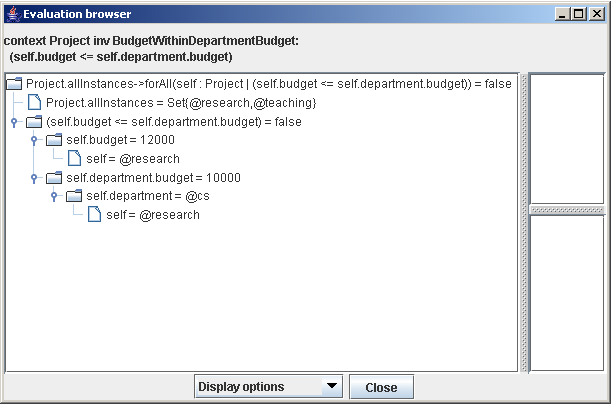
\includegraphics[scale=0.7]{Screenshots/GUI/EvalBrowserDemo.png}
\caption{Evaluation Browser showing the violated constraint}
\label{fig:EvalBrowserDemo}
\end{figure}\\
The root node in the evaluation browser shows the complete
expression and its result, which is false for the chosen invariant.
For each component of an expression there are child nodes displaying
the sub expressions and their results. You can see that the argument
expression of the $\mathit{forAll}$ quantifier is false, thus making the whole expression
result false. In this sub expression, the variable $\mathit{self}$ is bound to the object
$\mathit{research}$. The Evaluation Browser has helped to find out that it is the $\mathit{budget}$
attribute value of this object which causes the invariant to fail.
\section{Validating Pre- and Postconditions}
OCL provides special syntax for specifying pre- and postconditions
on operations in a UML model. Pre- and postconditions are constraints
that define a contract that an implementation of the operation has to fulfill.
A precondition must hold when an operation is called, a postcondition must be
true when the operation returns. The USE tool allows to validate pre- and postconditions
by simulating operation calls. The following describes how this feature works.
\subsection{Validating the Person \& Company Model}
We test the pre- and postconditions of the Person \& Company example
specified in section \ref{personCompanySpec}. First we
start the USE tool with the specification of the example model.
\begin{verbatim}
use> open ../examples/Documentation/Employee/Employee.use
compiling specification...
Model Employee (2 classes, 1 association, 0 invariants, 3 operations,
  7 pre-/postconditions)
\end{verbatim}
At the prompt, we enter the following commands to create two objects.
\begin{verbatim}
use> !create ibm : Company
use> !create joe : Person
use> !set joe.name := 'Joe'
use> !set joe.age := 23
\end{verbatim}
The current system state can be visualized with an
object diagram view in USE (see figure \ref{fig:EmployeeObjects}).\\
\begin{figure}[ht]
\centering
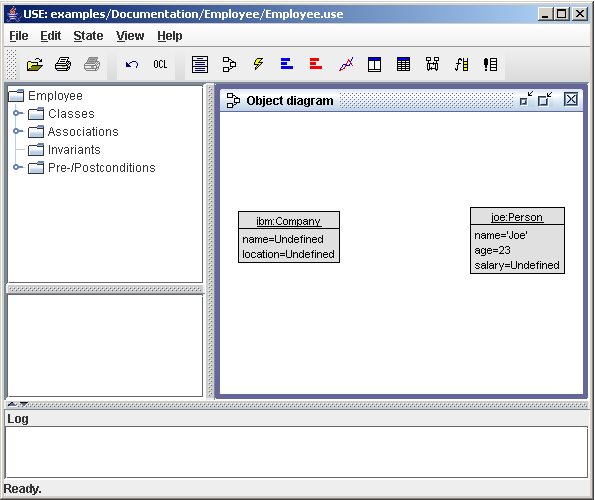
\includegraphics[scale=0.7]{Screenshots/GUI/EmployeeObjects.png}
\caption{Object diagram of the Person \& Company example}
\label{fig:EmployeeObjects}
\end{figure}\\
Next, we want to call the operation $\mathit{hire}$ on the company object to hire
$\mathit{joe}$ as a new employee.
\subsubsection{Calling Operations and Checking Preconditions}
Operation calls are initiated with the command \verb+openter+. Its syntax is
presented in section \ref{openterCmd}.
The following command shows the top level bindings of variables.
These variables can be used in expressions to refer to existing objects.
\begin{verbatim}
use> info vars
ibm : Company = @ibm
joe : Person = @joe
\end{verbatim}
We invoke the operation $\mathit{hire}$ on the receiver object $\mathit{ibm}$ and pass the object
$\mathit{joe}$ as parameter.
\begin{verbatim}
use> !openter ibm hire(joe)
precondition `hirePre1' is true
precondition `hirePre2' is true
\end{verbatim}
The openter command has the following effect.
\begin{description}
\item[1.] The source expression is evaluated to determine the receiver object.
\item[2.] The argument expressions are evaluated.
\item[3.] The variable $\mathit{self}$ is bound to the receiver object and the argument
values are bound to the formal parameters of the operation.
These bindings determine the local scope of the operation.
\item[4.] All preconditions specified for the operation are evaluated.
\item[5.] If all preconditions are satisfied, the current
system state is saved and the operation call is saved on a call stack.
\end{description}
In the example, the call of the operation $\mathit{hire}$ was successful because
both preconditions are satisfied. The stack of currently active
operations can be viewed by issuing the following command.
\begin{verbatim}
use> info opstack
active operations:
1. Company::hire(p : Person)
\end{verbatim}
We can verify the bindings of the $\mathit{self}$ variable and the formal parameter $p$ as follows.
\begin{verbatim}
use> info vars
ibm : Company = @ibm
joe : Person = @joe
p : Person = @joe
self : Company = @ibm
\end{verbatim}
\subsubsection{Operation Effects}
We can simulate the execution of an operation with
the usual USE primitives for changing a system state.
The postcondition of the $\mathit{hire}$ operation requires that
a $\mathit{WorksFor}$ link between the person and the company has to
be created. We also set the salary of the new employee.
\begin{verbatim}
use> !insert (p, ibm) into WorksFor
use> !set p.salary := 2000
\end{verbatim}
The object diagram in \ref{fig:EmployeeObjectsLinks}
shows the new system state with the
link between the $\mathit{Person}$ and $\mathit{Company}$ objects.
\begin{figure}[ht]
\centering
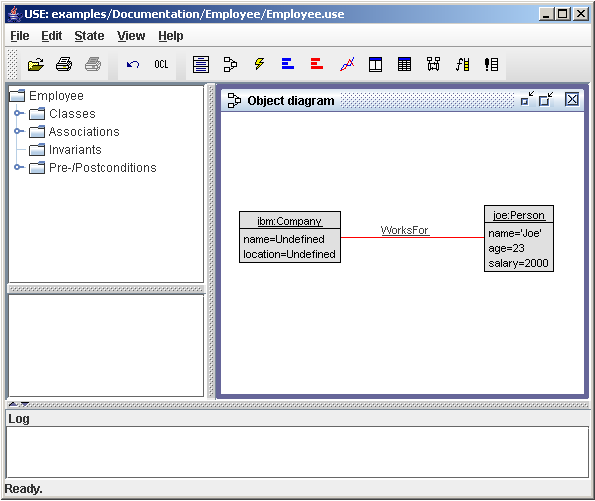
\includegraphics[scale=0.7]{Screenshots/GUI/EmployeeObjectsLinks.png}
\caption{Object diagram of the Person \& Company example after changing the state}
\label{fig:EmployeeObjectsLinks}
\end{figure}
\subsubsection{Exiting Operations and Checking Postconditions}
After generating all side effects of an operation,
we are ready to exit the operation and check its
postconditions. The command \verb+opexit+ simulates a
return from the currently active operation. The syntax is:\\\\
\verb+!opexit+ $\mathit{ReturnValExpr}$\\\\
The optional $\mathit{ReturnValExpr}$ is only required
for operations with a result value.
An example will be given later. The operation $\mathit{hire}$ specifies no result,
so we can just issue:
\begin{verbatim}
use> !opexit
postcondition `hirePost' is true
\end{verbatim}
The opexit command has the following effect.
\begin{description}
\item[1.] The currently active operation is popped from the call stack.
\item[2.] If an optional result value is given, it is
bound to the special OCL variable $\mathit{result}$.
\item[3.] All postconditions specified for the operation are
evaluated in context of the current system state and the
pre state saved at operation entry time.
\item[4.] All local variable bindings are removed.
\end{description}
In our example, the postcondition $\mathit{hirePost}$ is satisfied.\\\\
The operation has been removed from the call stack:
\begin{verbatim}
use> info opstack
no active operations.
\end{verbatim}
All variable bindings local to operations are removed on exit.
\begin{verbatim}
use> info vars
ibm : Company = @ibm
joe : Person = @joe
\end{verbatim}
Note that object names are elements of the top level bindings.
If you create new objects inside an operation call,
their names will still be available after exiting the operation.
\subsubsection{Result Values and References to the Previous State}
The operation $\mathit{raiseSalary}$ in class $\mathit{Person}$ is used for changing the
salary of an employee by a given rate.
The following constraints are added to the model specification.
\begin{verbatim}
context Person::raiseSalary(rate : Real) : Real
  post raiseSalaryPost:
    salary = salary@pre * (1.0 + rate)
  post resultPost:
    result = salary
\end{verbatim}
The first postcondition $\mathit{raiseSalaryPost}$ requires
that the new value of the salary attribute equals
a value that is computed in terms of the previous
value using the $\mathit{@pre}$ modifier. The second postcondition
$\mathit{resultPost}$ specifies that the result value of the operation
equals the new salary.\\\\
We call $\mathit{raiseSalary}$ on the new employee $\mathit{joe}$.
The rate $0.1$ is given to raise the salary by $10\%$.
\begin{verbatim}
use> !openter joe raiseSalary(0.1)
\end{verbatim}
The $\mathit{salary}$ attribute is assigned a new value with the \verb+set+ command.
\begin{verbatim}
use> !set self.salary := self.salary + self.salary * rate
\end{verbatim}
Since $\mathit{raiseSalary}$ is an operation with a return value,
we have to specify a result value on exit. This value
is bound to the OCL result variable when the postconditions are evaluated.
\begin{verbatim}
use> !opexit 2200
postcondition `raiseSalaryPost' is true
postcondition `resultPost' is true
\end{verbatim}
\subsubsection{Visualization as Sequence Diagram}
The USE tool can visualize a sequence of operation calls as a UML sequence diagram.
The screenshot in figure \ref{fig:EmployeeSequence} shows the sequence of calls for the example.
During a validation session the diagram is automatically updated on each operation call.
\begin{figure}[ht]
\centering
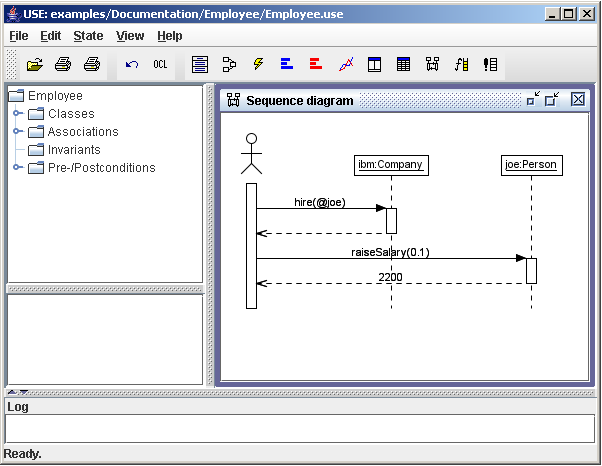
\includegraphics[scale=0.7]{Screenshots/GUI/EmployeeSequence.png}
\caption{Sequence diagram of the Person \& Company example}
\label{fig:EmployeeSequence}
\end{figure}
\subsection{An Example with oclIsNew}
The graph model specified in section \ref{graphsSpec} includes
constraints calling the operation $\mathit{oclIsNew}$.
We use the following command script for animating the model.
The script simulates three operation calls.
The first one is expected to succeed while the second
and third one should violate the postconditions.
\begin{verbatim}
!create n1 : Node

-- this call satisfies both postconditions
!openter n1 newTarget()
!create n2 : Node
!insert (n1,n2) into Edge
!opexit

-- postcondition oneNewTarget fails,
-- because n3 is not linked to n1
!openter n1 newTarget()
!create n3 : Node
!opexit

-- postcondition targetNodeIsNew fails,
-- because n3 has already been created above
!openter n1 newTarget()
!insert (n1,n3) into Edge
!opexit
\end{verbatim}
Here is the output of the USE tool confirming our expectations
about the success and failure of postconditions. Details during
the evaluation of failing postconditions provide hints about what went wrong.
\begin{verbatim}
$ use -nogui ../examples/Documentation/Graph/Graph.use
  ../examples/Documentation/Graph/Graph.cmd

use version 2.3.1-devel, Copyright (C) 1999-2006 University of Bremen
compiling specification...
Model Graph (1 class, 1 association, 0 invariants, 1 operation, 2 pre-/postconditions)
Graph.cmd> -- Opens the class diagram:
Graph.cmd> -- open examples/Documentation/Graph/Graph.use
Graph.cmd>
Graph.cmd> -- Creates the object diagram:
Graph.cmd> -- read examples/Documentation/Graph/Graph.cmd
Graph.cmd>
Graph.cmd> !create n1 : Node
Graph.cmd>
Graph.cmd> -- this call satisfies both postconditions
Graph.cmd> !openter n1 newTarget()
Graph.cmd> !create n2 : Node
Graph.cmd> !insert (n1,n2) into Edge
Graph.cmd> !opexit
postcondition `oneNewTarget' is true
postcondition `targetNodeIsNew' is true
Graph.cmd>
Graph.cmd> -- postcondition oneNewTarget fails,
because n3 is not linked to n1
Graph.cmd> !openter n1 newTarget()
Graph.cmd> !create n3 : Node
Graph.cmd> !opexit
postcondition `oneNewTarget' is false
evaluation results:
  self : Node = @n1
  self.target : Set(Node) = Set{@n2}
  self : Node = @n1
  self.target@pre : Set(Node) = Set{@n2}
  (self.target - self.target@pre) : Set(Node) = Set{}
  (self.target - self.target@pre)->size : Integer = 0
  1 : Integer = 1
  ((self.target - self.target@pre)->size = 1) : Boolean = false
postcondition `targetNodeIsNew' is true
Graph.cmd>
Graph.cmd> -- postcondition targetNodeIsNew fails,
because n3 has already been create above
Graph.cmd> !openter n1 newTarget()
Graph.cmd> !insert (n1,n3) into Edge
Graph.cmd> !opexit
postcondition `oneNewTarget' is true
postcondition `targetNodeIsNew' is false
evaluation results:
  self : Node = @n1
  self.target : Set(Node) = Set{@n2,@n3}
  self : Node = @n1
  self.target@pre : Set(Node) = Set{@n2}
  (self.target - self.target@pre) : Set(Node) = Set{@n3}
  n : Node = @n3
  n.oclIsNew : Boolean = false
  (self.target - self.target@pre)->forAll(n : Node | n.oclIsNew) : Boolean = false
Graph.cmd>
use>
\end{verbatim}
The screenshot in figure \ref{fig:GraphSequence} shows the sequence diagram automatically
generated from the example. Dashed return arrows in red
indicate that a postcondition failed on exit from an operation call.
\begin{figure}[ht]
\centering
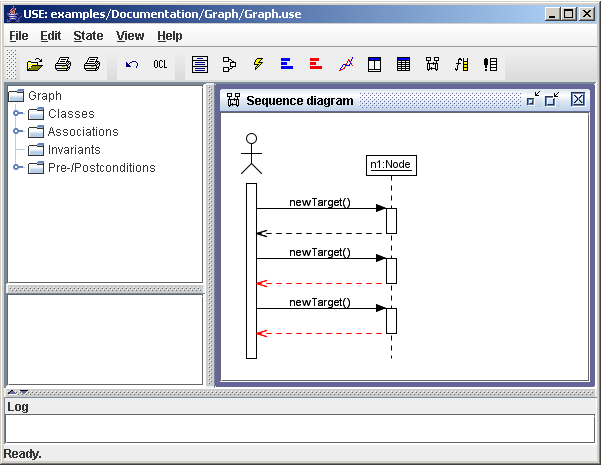
\includegraphics[scale=0.7]{Screenshots/GUI/GraphSequence.png}
\caption{Sequence diagram of the Graph example}
\label{fig:GraphSequence}
\end{figure}
\subsection{Nested Operation Calls}
The factorial example specified in section \ref{factorialSpec}
includes nested operation calls.
The following commands show the computation of 3!.
\begin{verbatim}
use> !create r : Rec
use> !openter r fac(3)
precondition `pre1' is true
use> !openter r fac(2)
precondition `pre1' is true
use> !openter r fac(1)
precondition `pre1' is true
\end{verbatim}
The call stack now looks like this.
\begin{verbatim}
use> info opstack
active operations:
1. Rec::fac(n : Integer) : Integer
2. Rec::fac(n : Integer) : Integer
3. Rec::fac(n : Integer) : Integer
\end{verbatim}
We exit the operations in reverse order and provide result values that satisfy the postcondition.
\begin{verbatim}
use> !opexit 1
postcondition `post1' is true
use> !opexit 2
postcondition `post1' is true
use> !opexit 6
postcondition `post1' is true
\end{verbatim}
The screenshot in figure \ref{fig:NestedSequence} shows the sequence
diagram automatically generated
from the example. Note the stacked activation frames
resulting from the recursion.
\begin{figure}[ht]
\centering
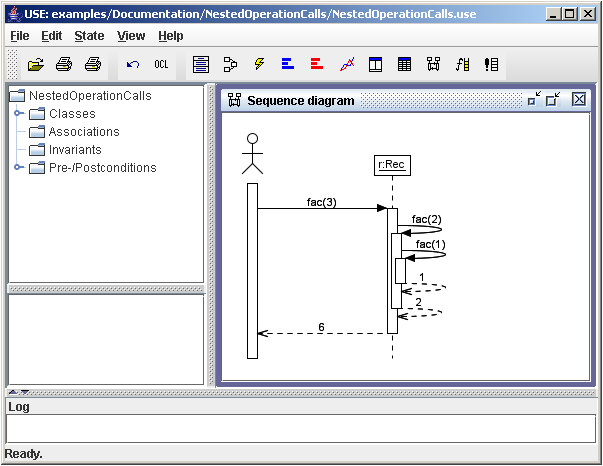
\includegraphics[scale=0.7]{Screenshots/GUI/NestedSequence.png}
\caption{Sequence diagram of the factorial example}
\label{fig:NestedSequence}
\end{figure}
\chapter{GUI Reference}
\section{The Menubar}
The symbols on the left side of the menu \index{Menubar} entries indicate that there is a corresponding button
available at the toolbar.
\subsection{File}
\subsubsection{Open Specification...}\label{openSpec}
Loads an available USE specification from file ($\mathit{filename}$\verb+.use+).
\subsubsection{Save Script...}
Saves all previously entered operation calls and
commands which changed the system state to file ($\mathit{filename}$\verb+.cmd+).
\subsubsection{Save Protocol...}
Saves a detailed protocol including many GUI and shell activities.
\subsubsection{Printer Setup...}
Opens a dialog with modifiable standard printer settings.
\subsubsection{Print Diagram...}\label{printDia}
Opens the printer window for printing the active diagram
with any desired settings.
\subsubsection{Print View...}\label{printView}
This function is enabled for sequence diagrams only.
It prints the visible part of the diagram.
For printing the whole sequence diagram, the
\verb+Print Diagram...+ function has to be used.
\subsubsection{Exit}
Quits the running USE system.
\subsection{Edit}
\subsubsection{Undo}\label{undo}
This function cancels the commands changing the system state step by step.
It makes no difference between GUI and shell commands.
\subsection{State}
\subsubsection{Create object...}
Shows all specified classes. After selecting a class,
any number of objects may be created by entering an unique object name.
\subsubsection{Evaluate OCL expression...}\label{evalExpr}
This function opens an evaluating window which consists of two parts.
In the upper part you can enter a OCL expression.
After evaluating the expression the lower part
shows the result with its type. The \verb+Clear+ button
clears the result information.
The \verb+Browser+ button opens the
evaluation browser for analyzing the entered expression and
its parts. If the evaluation browser is still opened and a new
expression is evaluated the browser will be actualized. If the
expression cannot be evaluated the browser window will be closed.
This also happens if the \verb+Clear+ button
is pressed.\\
The model elements like class names, role names
etc. may be integrated into the OCL expression.
If a system state is defined, object names may be used too.
\subsubsection{Check structure now}
This function checks if all multiplicities defined in the specification
are fulfilled by the system state.
\subsubsection{Check structure after every change}
Checks the structure for every command, which changed the system state.
\subsubsection{Reset}
Resets the system state to the empty state.
\subsection{View}
\subsubsection{Create}
Creates one of the available diagram views.
\subsubsection{Tile}
Arranges all displayed views next to each other.
\subsubsection{Close all}
Closes all displayed diagram views.
\subsection{Help}
\subsubsection{About...}
Opens the About window.
\section{Toolbar}
\begin{description}
\item 
\includegraphics[width=0.03\textwidth]{Pictures/Open.png} Open Specification (see section \ref{openSpec})
\item 
\includegraphics[width=0.03\textwidth]{Pictures/Print.png} Print Diagram (see section \ref{printDia})
\item 
\includegraphics[width=0.03\textwidth]{Pictures/Print.png} Print View (see section \ref{printView})
\item 
\includegraphics[width=0.03\textwidth]{Pictures/Undo.png} Undo (see section \ref{undo})
\item 
\includegraphics[width=0.03\textwidth]{Pictures/OCL.png} Evaluate OCL expression (see section \ref{evalExpr})
\item 
\includegraphics[width=0.03\textwidth]{Pictures/Class.png} Create Class Diagram View (see section \ref{classdiagramview})
\item 
\includegraphics[width=0.03\textwidth]{Pictures/ObjectDiagram.png} Create Object Diagram View (see section \ref{objectdiagramview})
\item 
\includegraphics[width=0.03\textwidth]{Pictures/InvariantView.png} Create Class Invariant View (see section \ref{classinvariantview})
\item 
\includegraphics[width=0.03\textwidth]{Pictures/ObjectCountView.png} Create Object Count View (see section \ref{objectcountview})
\item 
\includegraphics[width=0.03\textwidth]{Pictures/LinkCountView.png} Create Link Count View (see section \ref{linkcountview})
\item 
\includegraphics[width=0.03\textwidth]{Pictures/LineChartView.png} Create State Evolution View (see section \ref{stateevolutionview})
\item 
\includegraphics[width=0.03\textwidth]{Pictures/ObjectProperties.png} Create Object Properties View (see section \ref{objectpropertiesview})
\item 
\includegraphics[width=0.03\textwidth]{Pictures/ClassExtendView.png} Create Class Extend View (see section \ref{classextendview})
\item 
\includegraphics[width=0.03\textwidth]{Pictures/SequenceDiagram.png} Create Sequence Diagram View (see section \ref{sequencediagramview})
\item 
\includegraphics[width=0.03\textwidth]{Pictures/CallStack.png} Create Call Stack View (see section \ref{callstackview})
\item 
\includegraphics[width=0.03\textwidth]{Pictures/CmdList.png} Create Command List View (see section \ref{commandlistview})
\end{description}
\section{The Main Window}
\begin{figure}[ht]
\centering
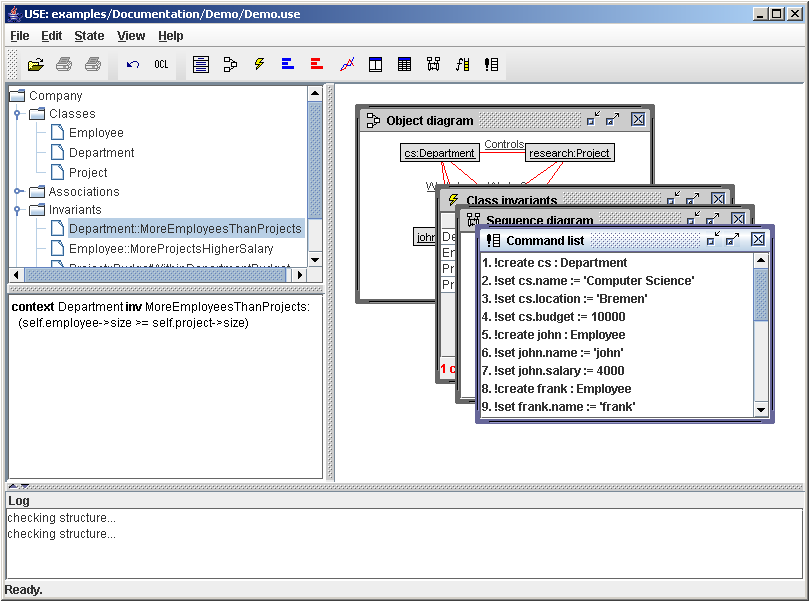
\includegraphics[scale=0.5]{Screenshots/GUI/Views/MainWindow.png}
\caption{Main window}
\label{fig:MainWindow}
\end{figure}
\subsection{Showing the diagram views}
The main part of the window shows the opened diagram views.
\subsection{Overview of the Specification}\label{specificationOverview}
The top left window represents the model browser. (see figure \ref{fig:OverviewOfSpec})
\begin{figure}[ht]
\centering
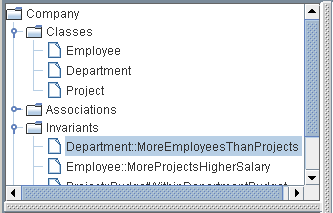
\includegraphics[scale=0.7]{Screenshots/GUI/Views/OverviewOfSpec.png}
\caption{Overview of the Specification}
\label{fig:OverviewOfSpec}
\end{figure}
It shows all defined classes,
associations, invariants and pre- and postconditions.
A right click into this part of the main window opens a context menu.
(see figure \ref{fig:OverviewOfSpecSort})
\begin{figure}[ht]
\centering
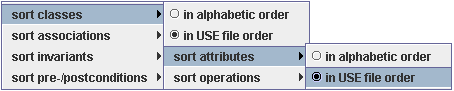
\includegraphics[scale=0.7]{Screenshots/GUI/Views/OverviewOfSpecSort.png}
\caption{Sorting}
\label{fig:OverviewOfSpecSort}
\end{figure}
The menu provides
the possibility to sort the specification elements e.g.
by name or \verb+use+ file order.
\subsection{Definition of the Specification elements}\label{low}
The window below the specification overview shows the definition of the
selected specification element as it is defined
in the .\verb+use+ file. (see figure \ref{fig:DefinitionOfSpec})
\begin{figure}[ht]
\centering
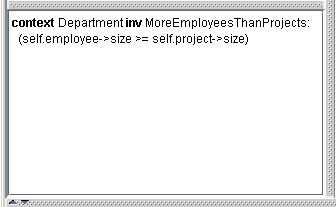
\includegraphics[scale=0.7]{Screenshots/GUI/Views/DefinitionOfSpec.png}
\caption{Definition of the specification elements}
\label{fig:DefinitionOfSpec}
\end{figure}
\subsection{Log window}\label{logWindow}
The lower part of the main window show a log of the system activities. (see figure \ref{fig:LogWindow})
It also lists
possible syntax resp. type check errors found in the loaded specification and
structural errors. Click right to clear the log window.
\begin{figure}[ht]
\centering
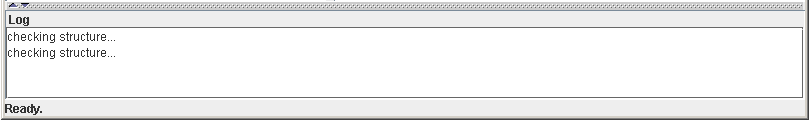
\includegraphics[scale=0.5]{Screenshots/GUI/Views/LogWindow.png}
\caption{Log window}
\label{fig:LogWindow}
\end{figure}
\subsection{Status and Tips}
A line on the bottom of the main window shows the current USE status and
tips with reference to the displayed diagrams. (see figure \ref{fig:StatusAndTips})
\begin{figure}[ht]
\centering

\includegraphics[scale=0.5]{Screenshots/GUI/Views/StatusAndTips.png}
\caption{Status and tips}
\label{fig:StatusAndTips}
\end{figure}
\section{Diagram Views}
There are different views, which can be used to analyze the current system state
with reference to the specification.
\subsection{General Functions}
Double click on the head of an active view to maximize the window resp. reduce it to the
previous size. There are three symbols in the upper right corner. They
minimize, maximize resp. reduce or close the active window.
\subsection{Class Diagram View}\label{classdiagramview}
This view shows the class diagram defined by the loaded specification. (see figure \ref{fig:ClassDiagramView})
\begin{figure}[ht]
\centering
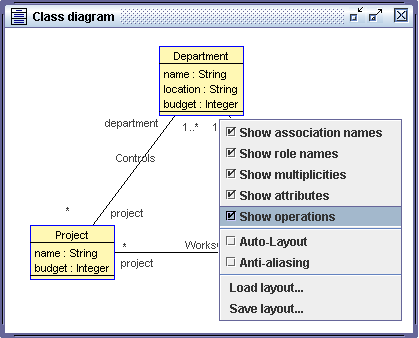
\includegraphics[scale=0.7]{Screenshots/GUI/Views/ClassDiagramView.png}
\caption{Class Diagram View (Employees, Departments and Projects Example)}
\label{fig:ClassDiagramView}
\end{figure}
It displays classes, attributes, operations, associations, inheritance, compositions, aggregations,
association classes, enumerations, role names and multiplicities.
Associations connect classes via edges. It is possible to create movable nodes
by double clicking an edge.
If an association is not 2 ary a diamond will connect the three or more participating classes.
A dashed line connects association classes to their edge.
You can move elements like classes, diamonds, role names, multiplicities
etc.. If you select an element, it appears orange. To mark
more than one element hold the shift button and select
the elements. The selected elements can be moved together.\\
Figure \ref{fig:ClassDiagramView} shows the context menu, which is
displayed after a right click. You can choose
if associations, role names, multiplicities, attributes
or operations should be displayed.
If you enable the \verb+Auto-Layout+ option, the system
tries to arrange the class diagram elements optimally.
The \verb+Anti-aliasing+ option switches the anti aliasing on
and off. It is possible to save resp. load an diagram layout
to resp. from file ($\mathit{filename}$\verb+.clt+).\\
If you select at least one Element, you can hide it or
all other elements but the selected ones. The \verb+Show+
command recovers the hidden elements. (see figure \ref{fig:ClassDiagramViewHideCrop})
\begin{figure}[ht]
\centering
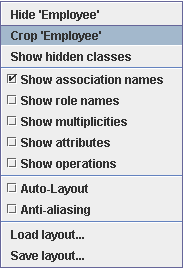
\includegraphics[scale=0.7]{Screenshots/GUI/Views/ClassDiagramViewHideCrop.png}
\caption{Class Diagram View - Context Menu with Hide, Crop, and Show}
\label{fig:ClassDiagramViewHideCrop}
\end{figure}
\subsection{Object Diagram View}\label{objectdiagramview}
The Object Diagram View shows the object diagram defined by the actual
system state. (see figure \ref{fig:ObjectDiagramView})
\begin{figure}[ht]
\centering
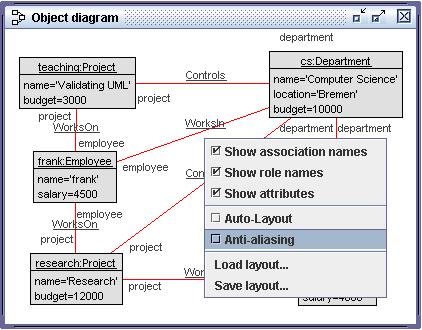
\includegraphics[scale=0.7]{Screenshots/GUI/Views/ObjectDiagramView.png}
\caption{Object Diagram View (Employees, Departments and Projects Example)}
\label{fig:ObjectDiagramView}
\end{figure}
It shows objects, attributes, attribute values, links, association names
and role names. The general functions are similar to
the Class Diagram View functions presented in section \ref{classdiagramview}.\\
Objects are displayed with object name and its type.
Double click on an object to open the object properties view.
(see figure \ref{objectpropertiesview})
Links are represented by a red line. Association names, role names and attributes
are optional elements. To display them, check the corresponding box in
the context menu, which is shown after a right click.
The \verb+Auto-Layout+, \verb+Anti-aliasing+, \verb+Load layout...+
and \verb+Save layout...+ functions are explained in section \ref{classdiagramview}.
\subsubsection{Creating and destroying objects without Shell commands}
The Model Browser (see section \ref{low}) shows all specified classes.
To create an instance of a class just drag the class name and drop
it into the object diagram view. This creates an object with undefined
attribute values.\\
You can destroy existing objects by selecting them. The context menu
shows a new \verb+Delete+ function, which will destroy the object and
the participating links. (see figure \ref{fig:ObjectDiagramViewAllFunctions})
\begin{figure}[ht]
\centering
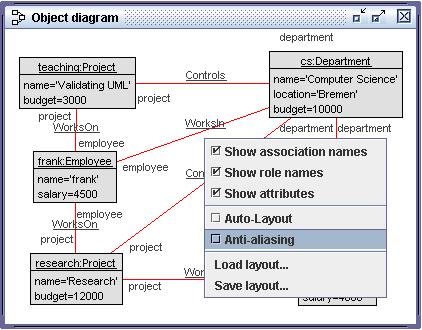
\includegraphics[scale=0.7]{Screenshots/GUI/Views/ObjectDiagramView.png}
\caption{Object Diagram View (Employees, Departments and Projects Example)}
\label{fig:ObjectDiagramViewAllFunctions}
\end{figure}
\subsubsection{Inserting and deleting links without shell commands}
To insert a link between two or more objects, select the objects
and open the context menu. Hold the shift button to select more than
one object. If there is an appropriate association the context menu shows
an \verb+insert+ command, which inserts
a link between the selected objects.
Association classes are created the same way.\\\\
Remove a link by selecting the involved objects. The context menu
shows a \verb+delete+ function.
\subsection{Class Invariant View}\label{classinvariantview}
Shows all invariants. (see figure \ref{fig:ClassInvariantView})
\begin{figure}[ht]
\centering
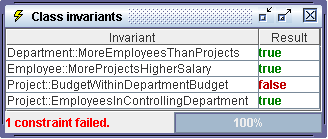
\includegraphics[scale=0.7]{Screenshots/GUI/Views/ClassInvariantView.png}
\caption{Class Invariant View (Employees, Departments and Projects Example)}
\label{fig:ClassInvariantView}
\end{figure}
If no instance of the invariant context
violates the corresponding invariant and no model inherent constraint
(see section \ref{modelinherent}) the view shows $\mathit{true}$.
If an objects violates a model inherent constraint it appears $N/A$.
$\mathit{false}$ appears otherwise.
The bottom of the window shows the number of violated invariants
in the actual system state. %(Was sagt die Prozentanzeige?).
A double click opens the evaluation browser analyzing the current invariant
with respect to the actual system state. (see section \ref{evaluationBrowserSec})
\subsection{Object Count View}\label{objectcountview}
Shows all classes on the left side and the number of their instances
on the right side. A bar chart shows an overview of the number of instances.
\begin{figure}[ht]
\centering
\includegraphics[scale=0.7]{Screenshots/GUI/Views/ObjectCountView.png}
\caption{Object Count View (Employees, Departments and Projects Example)}
\label{fig:ObjectCountView}
\end{figure}
\subsection{Link Count View}\label{linkcountview}
Shows all associations on the left side and the number of links
on the right side. A bar chart shows an overview of the number of links.
\begin{figure}[ht]
\centering
\includegraphics[scale=0.7]{Screenshots/GUI/Views/LinkCountView.png}
\caption{Link Count View (Employees, Departments and Projects Example)}
\label{fig:LinkCountView}
\end{figure}
\subsection{State Evolution View}\label{stateevolutionview}
Shows a line chart. (see figure \ref{fig:StateEvolutionView})
\begin{figure}[ht]
\centering
\includegraphics[scale=0.7]{Screenshots/GUI/Views/StateEvolutionView.png}
\caption{State Evolution View (Employees, Departments and Projects Example)}
\label{fig:StateEvolutionView}
\end{figure}
A blue line represents objects and
a red line represents links in the actual system state.
The y axis represents the number of
objects resp. links. The x axis represents the number of changes the user
made. Commands like \verb+set+ are considered as changes, too.
\subsection{Object Properties View}\label{objectpropertiesview}
The drop down menu of this view includes all objects. (see figure \ref{fig:ObjectPropertiesView})
\begin{figure}[ht]
\centering
\includegraphics[scale=0.7]{Screenshots/GUI/Views/ObjectPropertiesView.png}
\caption{Object Properties View (Employees, Departments and Projects Example)}
\label{fig:ObjectPropertiesView}
\end{figure}
If you choose an object its attributes and their values are displayed.
Double click on a value to change it. %(Was macht reset?)
The \verb+Apply+ button saves the changes.
\subsection{Class Extend View}\label{classextendview}
This view shows all objects of the selected class and their attribute values. (see figure \ref{fig:ClassExtendView})
\begin{figure}[ht]
\centering
\includegraphics[scale=0.7]{Screenshots/GUI/Views/ClassExtendView.png}
\caption{Class Extend View (Employees, Departments and Projects Example)}
\label{fig:ClassExtendView}
\end{figure}
A right click opens a context menu. You can switch on the
invariant results for each object and select a class.
An invariant receives a check symbol if the given object does not violate it.
Otherwise a cross appears.
If an object violates model inherent constraints the
invariant is not evaluated for this object. Then a question mark appears.
A double click opens the evaluation browser with the evaluation of
the selected invariant. It marks the sub formula for the corresponding object.
\subsection{Sequence Diagram View}\label{sequencediagramview}
\emph{Description will be available in the next document version.}
%Den Text f�r das Sequenzdiagramm muss ich noch einmal mit der Diplomarbeit
%von Antje Werner abgleichen. Damit auch alle Informationen
%enthalten sind.
\clearpage
\begin{figure}[ht]
\centering
\includegraphics[scale=0.5]{Screenshots/GUI/Views/SequenceDiagramView.png}
\caption{Sequence Diagram View (Graph Example)}
\label{fig:SequenceDiagramView}
\end{figure}
\begin{figure}[ht]
\centering
\includegraphics[scale=0.7]{Screenshots/GUI/Views/SeqDiagChooseCommands.png}
\caption{Choose Commands (Graph Example)}
\label{fig:SeqDiagChooseCommands}
\end{figure}
\begin{figure}[ht]
\centering
\includegraphics[scale=0.7]{Screenshots/GUI/Views/SeqDiagPropertiesDiagram.png}
\caption{Properties - Diagram (Graph Example)}
\label{fig:SeqDiagPropertiesDiagram}
\end{figure}
\begin{figure}[ht]
\centering
\includegraphics[scale=0.7]{Screenshots/GUI/Views/SeqDiagPropertiesLifelines.png}
\caption{Properties - Lifelines (Graph Example)}
\label{fig:SeqDiagPropertiesLifelines}
\end{figure}
\begin{figure}[ht]
\centering
\includegraphics[scale=0.7]{Screenshots/GUI/Views/SeqDiagPropertiesObjectBox.png}
\caption{Properties - Object Box (Graph Example)}
\label{fig:SeqDiagPropertiesObjectBox}
\end{figure}
\subsection{Call Stack View}\label{callstackview}
The Call Stack lists all operations which were called with
the \verb+openter+ command and did not terminate yet. They
terminate if you use the \verb+opexit+ command.
A right click opens the context menu. You can choose
if the operation signature or the concrete operation call
should be displayed.
\begin{figure}[ht]
\centering
\includegraphics[scale=0.7]{Screenshots/GUI/Views/CallStackView.png}
\caption{Call Stack View (Factorial Example)}
\label{fig:CallStackView}
\end{figure}
\subsection{Command List View}\label{commandlistview}
This view lists all commands defining the actual system state. (see figure \ref{fig:CommandListView})
\begin{figure}[ht]
\centering
\includegraphics[scale=0.7]{Screenshots/GUI/Views/CommandListView.png}
\caption{Command List View (Factorial Example)}
\label{fig:CommandListView}
\end{figure}
The \verb+reset+ command resets the system state and
empties the command list.
\section{Evaluation Browser}\label{evaluationBrowserSec}
You can open the Evaluation Browser via the Class Invariant View (see section \ref{classinvariantview}),
via the Class Extend View (see section \ref{classextendview}) or
the OCL Evaluation Window (see section \ref{evalExpr}). The figure \ref{fig:EvaluationBrowser}
shows the Evaluation Browser displaying the evaluation tree for the invariant
$\mathit{MoreEmployeesThanProjects}$ in the Employees, Departments and Projects example.\\
\begin{figure}[ht]
\centering
\includegraphics[scale=0.5]{Screenshots/GUI/EvaluationBrowser.png}
\caption{Evaluation Browser (Employees, Departments and Projects Example)}
\label{fig:EvaluationBrowser}
\end{figure}\\
A right click opens a large context menu. Its elements are explained in the following
subsections.
\subsection{Extended Evaluation}
You can select which OCL operations ($\mathit{exists}$, $\mathit{forAll}$,
$\mathit{and}$, $\mathit{or}$, $\mathit{implies}$) should be evaluated extendedly. (see
figure \ref{fig:EvaluationBrowserExtended}
\begin{figure}[ht]
\centering
\includegraphics[scale=0.7]{Screenshots/GUI/EvaluationBrowserMenuExtended.png}
\caption{Menu - Extended Evaluation}
\label{fig:EvaluationBrowserExtended}
\end{figure}
\subsubsection{exists}
Selecting the menu entry \verb+exists+ implicates that all $\mathit{exists}$ expressions
are evaluated extendedly. The extended evaluation does not stop if an element
fulfilling the body of the $\mathit{exists}$ expression was already found. The whole collection expression is
evaluated and all elements fulfilling the expression are displayed.
\subsubsection{forAll}
If you select the option \verb+forAll+ every $\mathit{forAll}$ expression is evaluated extendedly.
If an element does not fulfill the body of a $\mathit{forAll}$ expression, the extended evaluation does not stop, but
continues the iteration until the last element was regarded. All elements and their evaluation results are displayed.
\subsubsection{and}
The extended evaluation of $\mathit{and}$ expressions implies, that the right side
of an $\mathit{and}$ expression is evaluated even if the left side is not true.
The result of the right side is always displayed.
\subsubsection{or}
If the left side of an $\mathit{or}$ expression is true, USE normally stops the evaluation of
this expression. You can continue the evaluation even though the left side is already true, by
selecting the \verb+or+ option.
\subsubsection{implies}
The extended evaluation of $\mathit{implies}$ expressions evaluate the
conclusions even if the premises are false.
\subsubsection{all}
The \verb+all+ entry selects all options listed above.
\subsection{Variable Assignment Window}\label{variableAssignmentWindow}
If you switch on the Variable Assignment Window, it is displayed on the right side
of the evaluation Tree. \footnote{If the Subexpression Evaluation Window
is displayed too, the Variable Assignment Window appears above it.}
It shows all value assignments of the existing variables in the selected tree node.
The example in figure \ref{fig:EvaluationBrowser} shows the variable $\mathit{self}$ of type
$\mathit{Department}$ and its value $\mathit{@cs}$. The corresponding node
represents the expression $\mathit{@cs}.\mathit{project}\rightarrow\mathit{size}=2$.
\subsection{Subexpression Evaluation Window}
The Subexpression Evaluation Window is displayed on the right side of the evaluation tree
resp. below the Variable Assignment Window.
It shows the subexpressions of the marked tree node, which are evaluated in the
next step. The example in figure \ref{fig:EvaluationBrowser} marks a tree node with
expression $\mathit{@cs}.\mathit{project}\rightarrow\mathit{size}=2$. The navigation expression has to be evaluated
next. So the window shows the result of this subexpression:
$\mathit{Set}\{\mathit{@research},\mathit{@teaching}\}\rightarrow \mathit{size}=2$
\subsection{Tree Views}
You can choose between different tree views. They are listed in figure \ref{fig:EvaluationBrowserMenuTreeViews}
and explained below.
\begin{figure}[ht]
\centering
\includegraphics[scale=0.7]{Screenshots/GUI/EvaluationBrowserMenuTreeViews.png}
\caption{Menu - Tree Views}
\label{fig:EvaluationBrowserMenuTreeViews}
\end{figure}
\subsubsection{Late Variable Assignment}
In this view the tree nodes, showing the variable assignments, are the leafs of the tree.
(see figure \ref{fig:EvaluationBrowserLateAssignment})
\begin{figure}[ht]
\centering
\includegraphics[scale=0.7]{Screenshots/GUI/EvaluationBrowserLateAssignment.png}
\caption{Evaluation Browser - Late Variable Assignment (Employees, Departments and Projects Example)}
\label{fig:EvaluationBrowserLateAssignment}
\end{figure}
\subsubsection{Early Variable Assignment}
This view shows the variable assignment as soon as possible
in the evaluation tree. \footnote{Assignments can not be displayed until
the variables are bounded in the corresponding
OCL expression.} (see figure \ref{fig:EvaluationBrowserEarlyAssignment})
Simultaneous assignments are shown in the same node. They are separated by commas.
\begin{figure}[ht]
\centering
\includegraphics[scale=0.7]{Screenshots/GUI/EvaluationBrowserEarlyAssignment.png}
\caption{Evaluation Browser - Early Variable Assignment (Employees, Departments and Projects Example)}
\label{fig:EvaluationBrowserEarlyAssignment}
\end{figure}
\subsubsection{Variable Assignment \& Substitution}
The Variable Assignment \& Substitution view is a refinement of the previous
presented view. The variable names are substituted by their values.
(see figure \ref{fig:EvaluationBrowserAssignmentSubstitution})
\begin{figure}[ht]
\centering
\includegraphics[scale=0.7]{Screenshots/GUI/EvaluationBrowserAssignmentSubstitution.png}
\caption{Evaluation Browser - Variable Assignment \& Substitution (Employees, Departments and Projects Example)}
\label{fig:EvaluationBrowserAssignmentSubstitution}
\end{figure}
\subsubsection{Variable Substitution}
This view is similar to the Variable Assignment \& Substitution view, but
nodes with variable assignments are not displayed here. (see figure \ref{fig:EvaluationBrowserSubstitution})
\begin{figure}[ht]
\centering
\includegraphics[scale=0.7]{Screenshots/GUI/EvaluationBrowserSubstitution.png}
\caption{Evaluation Browser - Variable Substitution (Employees, Departments and Projects Example)}
\label{fig:EvaluationBrowserSubstitution}
\end{figure}
\subsubsection{No Variable Assignment}
This view does not display tree nodes with variable assignments, and does not substitute variables.
(see figure \ref{fig:EvaluationBrowserNoAssignment})
\begin{figure}[ht]
\centering
\includegraphics[scale=0.7]{Screenshots/GUI/EvaluationBrowserNoAssignment.png}
\caption{Evaluation Browser - No Variable Assignment (Employees, Departments and Projects Example)}
\label{fig:EvaluationBrowserNoAssignment}
\end{figure}
\subsection{True-False highlighting}
The context menu includes settings for colored and black/white highlighting of tree nodes.
(see figure \ref{fig:EvaluationBrowserMenuTrueFalse})
\begin{figure}[ht]
\centering
\includegraphics[scale=0.7]{Screenshots/GUI/EvaluationBrowserMenuTrueFalse.png}
\caption{Menu - True False Highlighting}
\label{fig:EvaluationBrowserMenuTrueFalse}
\end{figure}
Enabling highlighting changes the color resp. font of the tree nodes.
Nodes representing an expression, which evaluates to $\mathit{true}$, receives a green
color resp. a bold font, if the \verb+No colors+ option is switched on.
If an expression evaluates to $\mathit{false}$, the node
appears red resp. inverse colored.
Neutral nodes showing value assignments and undefined expressions are not highlighted.
You can choose between different highlighting modes. They are listed below.
\subsubsection{No Highlighting}
Deactivates the highlighting.
\subsubsection{Term Highlighting}
Highlights nodes of boolean type. (see figure \ref{fig:EvaluationBrowserTermHighlighting})
\begin{figure}[ht]
\centering
\includegraphics[scale=0.5]{Screenshots/GUI/EvaluationBrowserTermHighlighting.png}
\caption{Evaluation Browser - Term Highlighting (Employees, Departments and Projects Example)}
\label{fig:EvaluationBrowserTermHighlighting}
\end{figure}
\subsubsection{Subtree Highlighting}
Highlights nodes of boolean type and its child nodes if they have a different type.
Child nodes, which also have a boolean type, receive a color depending on their truth value.
The same highlighting rules are applied to their children.
(see figure \ref{fig:EvaluationBrowserSubtreeHighlighting})
\begin{figure}[ht]
\centering
\includegraphics[scale=0.5]{Screenshots/GUI/EvaluationBrowserSubtreeHighlighting.png}
\caption{Evaluation Browser - Subtree Highlighting (Employees, Departments and Projects Example)}
\label{fig:EvaluationBrowserSubtreeHighlighting}
\end{figure}
\subsubsection{Complete Subtree Highlighting}
The truth values of the immediate child nodes of the root specify the color of their subtrees.
(see figure \ref{fig:EvaluationBrowserCompleteHighlighting})
Other nodes have no influence on the subtree colors.
\begin{figure}[ht]
\centering
\includegraphics[scale=0.5]{Screenshots/GUI/EvaluationBrowserCompleteHighlighting.png}
\caption{Evaluation Browser - Complete Subtree Highlighting (Employees, Departments and Projects Example)}
\label{fig:EvaluationBrowserCompleteHighlighting}
\end{figure}
\subsection{Fit Width}
This command fits the width of the OCL expressions to the width of the Evaluation Browser Window.
You do not have to scroll horizontally.
\subsection{Default Configuration}
Restores the settings of the default configuration.
The command \verb+Set as default+ stores these settings. (see section \ref{setToDefault})
There is a USE configuration file \verb+etc/use.properties+ where
you can specify properties for all users.
You can also create a local \verb+.userc+ file in your home directory, which
overwrites or extends these settings. An example is shown below.
\begin{verbatim}
#Extended Evaluation Defaults
use.gui.view.evalbrowser.exists=false
use.gui.view.evalbrowser.forall=false
use.gui.view.evalbrowser.and=false
use.gui.view.evalbrowser.or=false
use.gui.view.evalbrowser.implies=false
#Extra-Windows
use.gui.view.evalbrowser.VarAssignmentWindow=false
use.gui.view.evalbrowser.SubExprSubstitutionWindow=false
#Tree-View Default
use.gui.view.evalbrowser.treeview=lateVarAssignment
#use.gui.view.evalbrowser.treeview=earlyVarAssignment
#use.gui.view.evalbrowser.treeview=substituteVarAssignment
#use.gui.view.evalbrowser.treeview=VarSubstitution
#use.gui.view.evalbrowser.treeview=noVarAssignment
#Highliting-Default
use.gui.view.evalbrowser.highliting=no
#use.gui.view.evalbrowser.highliting=term
#use.gui.view.evalbrowser.highliting=subtree
#use.gui.view.evalbrowser.highliting=complete
use.gui.view.evalbrowser.blackHighliting=false
\end{verbatim}
\subsection{Set to default}\label{setToDefault}
This commands opens the dialog shown in figure \ref{fig:EvaluationBrowserSetAsDefault}.
\begin{figure}[ht]
\centering
\includegraphics[scale=0.7]{Screenshots/GUI/EvaluationBrowserSetAsDefault.png}
\caption{Evaluation Browser - Set as Default}
\label{fig:EvaluationBrowserSetAsDefault}
\end{figure}
\subsubsection{For This session}
The current properties of the Evaluation Browser are saved, but not permanently.
They are saved as long as the USE process is running.
\subsubsection{For all sessions}
The settings are saved permanently by changing the \verb+.userc+ file
in your home directory.
\subsubsection{Cancel}
The dialog is closed without saving the actual configuration.
\subsection{Capture to File}
You can save the actual Evaluation Browser Window to file.
This command opens a save dialog where you can define the destination directory, the filename and
its format (\verb+PNG+, \verb+JPG+ or \verb+BMP+). \verb+PNG+ is the standard format.
\subsection{Shortcuts}
The above mentioned commands may be called by using shortcuts. The following
table shows the shortcuts and the corresponding commands.\\\\
\begin{tabular}{l|l}
{\bf Shortcut} & {\bf Command}\\\hline
Alt-x & Extended Evaluation (all)\\
Alt-v & Variable Assignment Window\\
Alt-e & Subexpression Evaluation Window\\
Alt-1..4 & Treeviews 1..4\\
Alt-0 & disable Highlighting\\
Alt-7..9 & Highlightings 1..3\\
Alt-f & Fit width\\
Alt-d & Default configuration\\
Alt-s & Set as default\\
Alt-c & Capture to file
\end{tabular}
\subsection{Context Menu}
You can click right on a tree node. If the node is closed, the context menu \ref{fig:EvaluationBrowserExpand}
is displayed.
\begin{figure}[ht]
\centering
\includegraphics[scale=0.7]{Screenshots/GUI/EvaluationBrowserExpand.png}
\caption{Evaluation Browser - Expand}
\label{fig:EvaluationBrowserExpand}
\end{figure}
Use the \verb+Expand+ function to open the node. The \verb+Expand all+ command opens the complete
subtree where the current node appears as root. The command \verb+Copy+ copies the OCL expression of the
marked node to clipboard.\\
The context menu changes, if the selected node is opened. (see \ref{fig:EvaluationBrowserCollapse})
\begin{figure}[ht]
\centering
\includegraphics[scale=0.7]{Screenshots/GUI/EvaluationBrowserCollapse.png}
\caption{Evaluation Browser - Collapse}
\label{fig:EvaluationBrowserCollapse}
\end{figure}
The node may be closed by using the \verb+Collapse+ function. But this command
does not close the child nodes. If you would like to close all child nodes too,
use the \verb+Collapse all+ function instead.
\subsection{Tree Display Menu}
The Tree Display Menu is a drop down menu shown in figure \ref{fig:EvaluationBrowserTreeDisplayAndClose}.
\begin{figure}[ht]
\centering
\includegraphics[scale=0.7]{Screenshots/GUI/EvaluationBrowserTreeDisplayAndClose.png}
\caption{Evaluation Browser - Tree Display Menu and Close button}
\label{fig:EvaluationBrowserTreeDisplayAndClose}
\end{figure}
It is located on the left side of the close button. The menu entries are listed below.
\subsubsection{Expand all}
Opens all nodes existing in the evaluation tree.
\subsubsection{Expand all true}
All displayed nodes of type boolean and their child nodes are opened if they evaluate to $\mathit{true}$.
\subsubsection{Expand all false}
All displayed nodes of type boolean and their child nodes are opened if they evaluate to $\mathit{false}$.
\subsubsection{Collapse}
This commands set the tree back to a state, where all nodes are folded up, but not the root.
\subsection{Hide Title}
The title of the Evaluation Browser shows the analyzed invariant and its definition. (see
figure \ref{fig:EvaluationBrowserTitle})
\begin{figure}[ht]
\centering
\includegraphics[scale=0.5]{Screenshots/GUI/EvaluationBrowserTitle.png}
\caption{Evaluation Browser - Title}
\label{fig:EvaluationBrowserTitle}
\end{figure}
If no invariant is actually analyzed, the expression of the root node is shown in the title.
You can hide the title by double click on it. If it is hidden you can double click at the top margin
to display the title again.
\subsection{Object Browser}
The Object Browser shows objects of user defined types, the valuation of their attributes,
their associations and the objects connected via links of the corresponding associations.
Double click on an object in the Variable Assignment Window to open the Object Browser.
(see section \ref{variableAssignmentWindow})\\
The figure \ref{fig:EvaluationBrowserObjectBrowser} shows the browser listing the information
about object \verb+@research+ in the Employees, Departments and Projects example.
\begin{figure}[ht]
\centering
\includegraphics[scale=0.7]{Screenshots/GUI/EvalBrowserObjectBrowser.png}
\caption{Evaluation Browser - Object Browser}
\label{fig:EvaluationBrowserObjectBrowser}
\end{figure}
The first column
shows its attributes, the second the corresponding values, the third shows its
associations and the fourth shows the objects which are connected to \verb+@research+
via links. You can navigate to connected objects by choosing them in a drop down menu.
Click left on the connected objects. This opens the menu, showing all
objects reachable from the current object.
After selecting the destination object, the Object Browser shows
its properties. (see figure \ref{fig:EvaluationBrowserObjectBrowserDropDown})
\begin{figure}[ht]
\centering
\includegraphics[scale=0.7]{Screenshots/GUI/EvalBrowserObjectBrowserDropDown.png}
\caption{Evaluation Browser - Object Browser with Dropdown menu}
\label{fig:EvaluationBrowserObjectBrowserDropDown}
\end{figure}
\chapter{Shell Reference}
\section{Commands}\label{ShellCommands}
\subsection{Overview of the Shell commands}
Prints all available commands and a synopsis of their description.
\begin{description}
\item[Syntax:] \verb+help+
\end{description}
\subsection{Help about a specific Shell command}
Prints the syntax for the use of command $\mathit{cmd}$ and its description with synopsis.
\begin{description}
\item[Syntax:] \verb+help+ $\mathit{cmd}$
\item[Example:] \verb+help !create+
\end{description}
\subsection{Compile and evaluate an OCL expression}
Compiles and evaluates the expression $\mathit{OclExpr}$. This Shell command
is comparable to the function of the Evaluation Window in the GUI. (see section \ref{evalExpr})
\begin{description}
\item[Syntax:] \verb+?+ $\mathit{OclExpr}$
\item[Example:] The simple expression $2=2$ has to be evaluated.
\begin{description}
\item[User input:]\verb+? 2=2+
\item[Result:] The result shown in the Shell.
\begin{verbatim}
-> true : Boolean
\end{verbatim}
\end{description}
\end{description}
\subsection{Compile and evaluate an OCL expression (verbose)}
Compiles and evaluates the Expression $\mathit{OclExpr}$ with verbose output of
subexpression results. After evaluating the expression the Evaluation Browser is displayed.
It shows the evaluation tree for $\mathit{OclExpr}$.
\begin{description}
\item[Syntax:] \verb+??+ $\mathit{OclExpr}$
\item[Example:] The simple expression $2=2$ has to be evaluated in verbose mode.
\begin{description}
\item[User input:]\verb+?? 2=2+
\item[Result:] The result shown in the Shell.
\begin{verbatim}
Detailed results of subexpressions:
  2 : Integer = 2
  2 : Integer = 2
  (2 = 2) : Boolean = true
-> true : Boolean
\end{verbatim}
\end{description}
\end{description}
\subsection{Compile an OCL expression and show its static type}
Compiles the expression $\mathit{OclExpr}$ and shows its static type.
\begin{description}
\item[Syntax:] \verb+:+ $\mathit{OclExpr}$
\item[Example:] The type of the expression $2=2$ has to be identified.
\begin{description}
\item[User input:]\verb+: 2=2+
\item[Result:] The result shown in the Shell.
\begin{verbatim}
-> Boolean
\end{verbatim}
\end{description}
\end{description}
\subsection{Enter OCL expressions over multiple lines}
Use \verb+\+ to enter a multiline mode. Finish with a '.' on a single line.
In multiline mode an OCL expression may be split into several lines.
\begin{description}
\item[Syntax:] The OCL expression is split into $n$ parts. Lines may be blank.
\begin{verbatim}
\
OclExprPart1
OclExprPart2
...
OclExprPartn
.
\end{verbatim}
\item[Example:] The Expression $2=2$ is split into 3 lines. One of them is a blank line.
\begin{description}
\item[User Input:] ~
\begin{verbatim}
\
?2

=2
.
\end{verbatim}
\item[Result:] The result shown in the Shell.
\begin{verbatim}
-> true : Boolean
\end{verbatim}
\end{description}
\end{description}
\subsection{Create objects}\label{createObjects}
Creates one or more objects of a given class or associationclass.
The $\mathit{newIdList}$ has to include at least one object name. These names
identify the new objects of the type $\mathit{class}$. If $\mathit{class}$ is an
association class the link ends given with $\mathit{idList}$ have to be specified with
the keyword \verb+between+.
The order of the names in $\mathit{idList}$ must conform to the definition of
the associationclass.
\begin{description}
\item[Syntax:] \verb+!create+ $\mathit{newIdList}$ \verb+:+ $\mathit{class}$ $[$\verb+between (+ $\mathit{IdList}$ \verb+)+$]$
\item[Example for classes:] The following commands create three objects for
the class $\mathit{Apple}$ and one for the classes $\mathit{Lemon}$ and $\mathit{Banana}$.
\begin{description}
\item[User input:] The user input.
\begin{verbatim}
!create greenApple, redApple, yellowApple : Apple
!create bigLemon : Lemon
!create banana : Banana
\end{verbatim}
\end{description}
\item[Example for association classes:] This example creates an instance of the associationclass $\mathit{FruitSalad}$.
The actual link ends are the existing objects $\mathit{banana}$ with type
$\mathit{Banana}$ and $\mathit{redApple}$ with type $\mathit{Apple}$.
\begin{description}
\item[User input:] The Shell command.
\begin{verbatim}
!create smallSalad : FruitSalad between (banana, redApple)
\end{verbatim}
\end{description}
\end{description}
\subsection{Destroy objects}
Destroys the objects given by the $\mathit{idList}$, which includes at least one object name.
If the destroyed object is a link end, the corresponding link is deleted resp. the associationclass object is
destroyed.
\begin{description}
\item[Syntax:] \verb+!destroy+ $\mathit{idList}$
\item[Example:] The example destroys two objects.
\begin{description}
\item[User input:] \verb+!destroy greenApple, smallSalad+
\end{description}
\end{description}
\subsection{Insert a link into an association}\label{insertInto}
Inserts a link between the objects in the $\mathit{idList}$ into the association $\mathit{assoc}$.
\begin{description}
\item[Syntax:] \verb+!insert+ $\mathit{idList}$ \verb+into+ $\mathit{assoc}$
\item[Example:] This command inserts a link into the 3 ary association $\mathit{Ingredients}$.
The second link end must have the type $\mathit{Orange}$. This is an abstract class. It cannot be instantiated.
$\mathit{Apple}$ is a subtype of this class. That means we may use the object $\mathit{yellowApple}$.
\begin{description}
\item[User input:] The Shell command.
\begin{verbatim}
!insert (redApple, yellowApple, bigLemon) into Ingredients
\end{verbatim}
\end{description}
\end{description}
\subsection{Delete a link from an association}
Deletes the link between the objects in the $\mathit{idList}$ from the association $\mathit{assoc}$.
\begin{description}
\item[Syntax:] \verb+!delete+ $\mathit{idList}$ \verb+from+ $\mathit{assoc}$
\item[Example:] This command deletes the link inserted in section \ref{insertInto}.
\begin{description}
\item[User input:] The Shell command.
\begin{verbatim}
!delete (redApple, yellowApple, bigLemon) from Ingredients
\end{verbatim}
\end{description}
\end{description}
\subsection{Set an attribute value of an object}
Sets the attribute $\mathit{attr}$ of the object $\mathit{obj}$ to a new value given by
$\mathit{OclExpr}$.
\begin{description}
\item[Syntax:] \verb+!set+ $\mathit{obj}$\verb+.+$\mathit{attr}$ \verb+:=+ $\mathit{OclExpr}$
\item[Example:] Both commands set the boolean attribute of object $\mathit{redApple}$
to true. It inherits the $\mathit{juice}$ attribute from $\mathit{Orange}$.
\begin{description}
\item[User input:] Two shell commands.
\begin{verbatim}
!set redApple.juice := 2=2
!set redApple.juice := true
\end{verbatim}
\end{description}
\end{description}
\subsection{Enter object operation}\label{openterCmd}
Invokes an operation with the name $\mathit{OpName}$ on the object $\mathit{ObjExpr}$.
If the operation has $n$ parameters, the $\mathit{ExprList}$ includes $n$
expressions which evaluate to the corresponding values.
If there is more than one operation call a call stack is used to remember the
entered operations. The deepest call has to be exited first.
\begin{description}
\item[Syntax:] \verb+!openter + $\mathit{ObjExpr~}$ $\mathit{OpName}$\verb+(+$\mathit{ExprList}$\verb+)+
\item[Example without parameters:] The object $\mathit{banana}$ is an instance of class $\mathit{Banana}$ which
defines the operation $\mathit{peel}$. This operation has no parameters.
\begin{description}
\item[User input:] \verb+!openter banana peel()+
\item[Result:] The preconditions are checked.
\begin{verbatim}
precondition `pre1' is true
\end{verbatim}
\end{description}
\item[Example with formal parameter:] The operation $\mathit{squeeze}$ is invoked on
object $\mathit{bigLemon}$. It has one explicitly defined parameter of type $\mathit{Integer}$.
\begin{description}
\item[User input:] \verb+!openter bigLemon squeeze(11)+
\item[Result:] The second precondition is false because the argument is greater than
10. The operation call is canceled.
\begin{verbatim}
precondition `pre2' is true
precondition `lessThanTenOranges' is false
\end{verbatim}
\item[User input:] \verb+!openter bigLemon squeeze(3)+
\item[Result:] Both preconditions are true.
\begin{verbatim}
precondition `pre2' is true
precondition `lessThanTenOranges' is true
\end{verbatim}
\end{description}
\end{description}
\subsection{Exit least recently entered operation}
This command exits the least recently entered operation, i.e. the top of the call stack.
If the operation has a return value it has to be specified behind the \verb+opexit+ command.
\begin{description}
\item[Syntax:] \verb+!opexit + $\mathit{ReturnValExpr}$
\item[Example - second call:] The operation $\mathit{squeeze}$ is the least recently entered
operation. Its return value has to be of type $\mathit{Integer}$.
\begin{description}
\item[User input:] \verb+ !opexit 20+
\item[Result:] The postconditions are checked.
\begin{verbatim}
postcondition `alwaysTrue' is true
\end{verbatim}
\end{description}
\item[Example - first call:] The operation $\mathit{peel}$ has been called before.
It can be exited now. The result value has to be a $\mathit{String}$.
\begin{description}
\item[User input:] \verb+!opexit 'failure'+
\item[Result:] One postcondition is false because the result value has to be $'\mathit{theResult}'$.
Even though the result value is wrong the operation is exited.
\begin{verbatim}
postcondition `post1' is true
postcondition `post2' is false
evaluation results:
  result : String = 'failure'
  'theResult' : String = 'theResult'
  (result = 'theResult') : Boolean = false
\end{verbatim}
\item[User input:] \verb+!openter 'theResult'+
\item[Result:] If we exit this operation with the right result value both preconditions appear true.
\begin{verbatim}
postcondition `post1' is true
postcondition `post2' is true
\end{verbatim}
\end{description}
\end{description}
\subsection{Check integrity constraints}
The command checks the structure, i.e. the multiplicity constraints and the invariant constraints.
There are four optional parameters. \verb+-v+ enables the verbose output of the subexpression results for violated
invariants. The option \verb+-d+ shows which instances cause an invariant to fail. The option
\verb+-a+ checks all invariants
including the ones loaded by the generator. You can specify which invariants should
be checked by entering an $\mathit{invList}$.
Use the following invariant signature: $\mathit{context}$\verb+::+$\mathit{invName}$.
The signatures have to be separated with a blank.
\begin{description}
\item[Syntax:] \verb+check + $[$\verb+-v+$]~[$\verb+-d+$]~[$\verb+-a+$~|~\mathit{invList}~]$
\item[Example without options:]~
\begin{description}
\item[User input:] \verb+check+
\item[Result:]The result shows several multiplicity constraint violations,
because the example script does not create enough links. One invariant is violated
in the current system state.
\begin{verbatim}
checking structure...
Multiplicity constraint violation in association `AppleSpritzer':
  Object `yellowApple' of class `Apple'
    is connected to 0 objects of class `Lemon' via role `flavor'
  but the multiplicity is specified as `1..8,10,15..*'.
...
Multiplicity constraint violation in association `Ingredients':
  Objects `yellowApple, redApple'
    are connected to 0 objects of class `Lemon'
  but the multiplicity is specified as `1..*'.
checking invariants...
checking invariant (1) `Orange::OrangeInv': OK.
checking invariant (2) `Orange::alwaysTrue': OK.
checking invariant (3) `Orange::inv2': FAILED.
  -> false : Boolean
checking invariant (4) `Peach::inv1': OK.
checking invariant (5) `Peach::neverViolated': OK.
checked 5 invariants in 0.046s, 1 failure.
\end{verbatim}
\end{description}
\item[Example with options:]~
\begin{description}
\item[User input:] \verb+check -d+
\item[Result:] The option \verb+-d+ shows, that $\mathit{redApple}$ and $\mathit{yellowApple}$
violate the invariant $\mathit{inv2}$.
with these options.
\begin{verbatim}
...
checking invariant (3) `Orange::inv2': FAILED.
  -> false : Boolean
Instances of Orange violating the invariant:
  -> Set{@redApple,@yellowApple} : Set(Apple)
...
\end{verbatim}
\end{description}
\end{description}
\subsection{Activate single-step mode}
This command activates the single step mode to read in a script
step by step.
\begin{description}
\item[Syntax:] \verb+step on+
\item[Example:] Read in the script.
\begin{description}
\item[User input:] Enter the step on mode and open the script.
\begin{verbatim}
use> step on
Step mode turned on.
use> open ../examples/Documentation/ExampleSpecification/ExampleScript.cmd
[step mode: `return' continues, `escape' followed by `return'
exits step mode.]
\end{verbatim}
\item[Result:] Now you can press return to read in the script command by command.
\end{description}
\end{description}
\subsection{Read information from File}
Reads information from a file. It may be a USE specification ($\mathit{fileName}$\verb+.use+),
a command file ($\mathit{fileName}$\verb+.cmd+), or an invariants file ($\mathit{fileName}$\verb+.invs+).
If a command file is read in, every line is shown in the Shell. You have to load a specification before you can read in command files.
The \verb+-q+ option allows a quiet reading.
If the filename is in the root directory of USE, there is no need to enter
the path. If the file exists in a subdirectory of the USE root directory (usually named \verb+use-+$\mathit{version}$),
you have to enter the sub path beginning at the USE root. (see example)
If the file does not exist in the USE directory you have to enter the whole path.
\begin{description}
\item[Syntax:] \verb+open+ $[\mathit{path}]$ $\mathit{fileName}$\verb+.+$(~$\verb+use+$~|~$\verb+cmd+$~|~$\verb+invs+$~)$
\item[Example file in USE sub directory:] Read in a specification existing in a subdirectory
of USE.
\begin{description}
\item[User input:]\verb+open ../examples/Documentation/Demo/Demo.use+
\item[Result:]~
\begin{verbatim}
compiling specification...
Model Company (3 classes, 3 associations, 4 invariants,
0 operations, 0 pre-/postconditions)
\end{verbatim}
\end{description}
\item[Example file not in USE directory:] Read in a specification.
\begin{description}
\item[User input:]\verb+open /home/opti/ExampleSpecification.use+
\item[Result:]~
\begin{verbatim}
compiling specification...
Model Fruits (6 classes, 3 associations, 5 invariants,
3 operations, 6 pre-/postconditions)
\end{verbatim}
\end{description}
\end{description}
\subsection{Reset system to empty state}
Resets the USE system state to an empty state. All objects and links are deleted.
\begin{description}
\item[Syntax:] \verb+reset+
\end{description}
\subsection{Exit USE}
Enter \verb+q+, \verb+quit+ or \verb+exit+ to exit USE.
\begin{description}
\item[Syntax:] $(~$\verb+q+$~|~$\verb+quit+$~|~$\verb+exit+$~)$
\end{description}
\subsection{Undo last state manipulation command}
Undoes the last state manipulation command.
\begin{description}
\item[Syntax:] \verb+undo+
\end{description}
\subsection{Print info about a class}
Prints information about a class existing in the specification.
\begin{description}
\item[Syntax:] \verb+info class+ $\mathit{className}$
\item[Example:] Get information about the $\mathit{Apple}$.
\begin{description}
\item[User input:]\verb+info class Apple+
\item[Result:] The result shown in the Shell.
\begin{verbatim}
class Apple < Lemon,Orange
end
2 objects of this class in current state.
\end{verbatim}
\end{description}
\end{description}
\subsection{Print info about loaded model}
Prints all information about the loaded model (classes, associations, constraints).
\begin{description}
\item[Syntax:] \verb+info model+
\item[Example:] Information about the example model.
\begin{description}
\item[User input:]\verb+info model+
\end{description}
\end{description}
\subsection{Print info about current system state}
Prints information about the current system state.
Shows how many objects and links are created.
\begin{description}
\item[Syntax:] \verb+info state+
\item[Example:] Information about the current state.
\begin{description}
\item[User input:]\verb+info state+
\item[Result:] The result shown in the Shell.
\begin{verbatim}
State: state#4
class      : #objects + #objects in subclasses
----------------------------------------------
Apple      :        2                        2
Banana     :        1                        1
FruitSalad :        0                        0
Lemon      :        1                        4
(Orange)   :        0                        2
Peach      :        0                        0
----------------------------------------------
total      :        4

association   : #links
----------------------
AppleSpritzer :      0
FruitSalad    :      0
Ingredients   :      0
----------------------
total         :      0
\end{verbatim}
\end{description}
\end{description}
\subsection{Print currently active operations}
Prints all operations, which did not terminate yet, i.e. the operation call stack.
\begin{description}
\item[Syntax:] \verb+info opstack+
\item[Example:] Invokes an operation and requests information about the operation stack.
\begin{description}
\item[User input:]~
\begin{verbatim}
use> !openter bigLemon squeeze(1)
precondition `pre2' is true
precondition `lessThanTenOranges' is true
use> info opstack
\end{verbatim}
\item[Result:] The result shown in the Shell.
\begin{verbatim}
active operations:
1. Lemon::squeeze(i : Integer) : Integer | bigLemon.squeeze(1)
\end{verbatim}
\end{description}
\end{description}
\subsection{Print internal program info}
Prints information about the USE process (i.e., memory usage).
\begin{description}
\item[Syntax:] \verb+info prog+
\item[Example:]
\begin{description}
\item[User input:]\verb+info prog+
\item[Result:] The result shown in the Shell.
\begin{verbatim}
(mem: 27% = 793.800 bytes free, 2.916.352 bytes total)
\end{verbatim}
\end{description}
\end{description}
\subsection{Print information about global variables}
Prints information about global variables.
\begin{description}
\item[Syntax:] \verb+info vars+
\item[Example:] The simple expression $2=2$ has to be evaluated.
\begin{description}
\item[User input:]\verb+info vars+
\item[Result:] The result shown in the Shell.
\begin{verbatim}
redApple : Apple = @redApple
yellowApple : Apple = @yellowApple
bigLemon : Lemon = @bigLemon
banana : Banana = @banana
i : Integer = 1
self : Lemon = @bigLemon
\end{verbatim}
\end{description}
\end{description}
\section{Generator}
\emph{Description will be available in the next document version.}
\chapter{OCL Standard Operations}
The OCL Standard operations are described following \cite{kyas:phd}.
\section{Object Types}
\subsection{Equality}
$=(y:\mathit{OclAny}):\mathit{Boolean}$ represents equality
between objects. It evaluates to true if $\mathit{self}$ is the same as $y$.\\
{\bf Notation:} $\mathit{self}$\verb+=+$y$
\subsection{Inequality}
$<>(y:\mathit{OclAny}):\mathit{Boolean}\stackrel{\mathit{def}}{=}\mathit{not}\ (
\mathit{self}=y)$ represents inequality between objects.\\
{\bf Notation:} $\mathit{self}$\verb+<>+$y$
\subsection{isUndefined}
$\mathit{isUndefined}():\mathit{Boolean}$ evaluates to true, if the
callee is undefined.\\
{\bf Notation:} $\mathit{self}$\verb+.isUndefined()+
\subsection{oclIsNew}
$\mathit{oclIsNew}():\mathit{Boolean}\stackrel{\mathit{def}}{=}
\mathit{self}@\mathit{pre}.\mathit{isUndefined}()$ can only be used
in a postcondition and states that the object has
been newly created during the execution of an operation.\\
{\bf Notation:} $\mathit{self}$\verb+.oclIsNew()+
\subsection{oclAsType}
$\mathit{oclAsType}(T):T$ is a ``cast'' or ``retyping'' expression,
  evaluating to the value of the callee, if it is an instance of $T$,
  and to $\mathit{Undefined}$ otherwise.\\
  {\bf Notation:} $\mathit{self}$\verb+.oclAsType(+$T$\verb+)+
\subsection{oclIsTypeOf}
$\mathit{oclIsTypeOf}(T):\mathit{Boolean}$ evaluates to $\mathit{true}$ if the
callee is an instance of type $T$.\\
{\bf Notation:} $\mathit{self}$\verb+.oclIsTypeOf(+$T$\verb+)+
\subsection{oclIsKindOf}
$\mathit{oclIsKindOf}(T):\mathit{Boolean}$ evaluates to $\mathit{true}$ if the
callee is
  an instance of type $T$ or one of $T$s subtypes, that is, the callee
  conforms to the type $T$.\\
  {\bf Notation:} $\mathit{self}$\verb+.isKindOf(+$T$\verb+)+
\section{Boolean Types}
\begin{tabular}{cc|ccccc}\hline
  $a$ & $b$ & $\mathit{not}\ b$ & $a\ \mathit{and}\ b$ & $a\
  \mathit{or}\ b$ & $a\ \mathit{implies}\ b$ & $a\ \mathit{xor}\ b$\\ \hline
  $\mathit{true}$ & $\mathit{true}$ & $\mathit{false}$ & $\mathit{true}$ & $\mathit{true}$ & $\mathit{true}$ & $\mathit{false}$ \\
  $\mathit{true}$ & $\mathit{false}$ & $\mathit{true}$ & $\mathit{false}$ & $\mathit{true}$ & $\mathit{false}$ & $\mathit{true}$ \\
  $\mathit{true}$ & $\bot$ & $\bot$ & $\bot$ & $\mathit{true}$ & $\bot$ & $\bot$ \\
  $\mathit{false}$ & $\mathit{true}$ & $\mathit{false}$ & $\mathit{false}$ & $\mathit{true}$ & $\mathit{true}$ & $\mathit{true}$ \\
  $\mathit{false}$ & $\mathit{false}$ & $\mathit{true}$ & $\mathit{false}$ & $\mathit{false}$ & $\mathit{true}$ & $\mathit{false}$ \\
  $\mathit{false}$ & $\bot$ & $\bot$ & $\mathit{false}$ & $\bot$ & $\mathit{true}$ & $\bot$ \\
  $\bot$ & $\mathit{true}$ & $\mathit{false}$ & $\bot$ & $\mathit{true}$ & $\mathit{true}$ & $\bot$ \\
  $\bot$ & $\mathit{false}$ & $\mathit{true}$ & $\mathit{false}$ & $\bot$ & $\bot$ & $\bot$ \\
  $\bot$ & $\bot$ & $\bot$ & $\bot$ & $\bot$ & $\bot$ & $\bot$ \\ \hline
\end{tabular}
\section{Real}
\subsection{Addition}
$+(y:\mathit{Real}):\mathit{Real}$ describes the sum of $\mathit{self}$ and $y$.\\
{\bf Notation:} $\mathit{self}$\verb-+-$y$
\subsection{Subtraction}
$-(y:\mathit{Real}):\mathit{Real}$ describes the difference between
$\mathit{self}$
  and $y$.\\
  {\bf Notation:} $\mathit{self}$\verb+-+$y$
\subsection{Multiplication}
$*(y:\mathit{Real}):\mathit{Real}$ describes the product of $\mathit{self}$ and
$y$.\\
{\bf Notation:} $\mathit{self}$\verb+*+$y$
\subsection{Division}
$/(y:\mathit{Real}):\mathit{Real}$ describes the quotient of $\mathit{self}$
and $y$.\\
{\bf Notation:} $\mathit{self}$\verb+/+$y$
\subsection{Negation}
$-():\mathit{Real}\stackrel{def}{=} 0-\mathit{self}$ describes the negation
of $\mathit{self}$.\\
{\bf Notation:} \verb+-+$\mathit{self}$
\subsection{Less}
$<(y:\mathit{Real}):\mathit{Boolean}$ evaluates to $\mathit{true}$,
if the value of
  $\mathit{self}$ is less than the value of $y$.  It evaluates to $\mathit{false}$, if
  the value of $\mathit{self}$ is equal to or greater than the value of $y$.
  In any other case, it is undefined.\\
  {\bf Notation:} $\mathit{self}$\verb+<+$y$
\subsection{Greater}
$>(y:\mathit{Real}):\mathit{Boolean}$ evaluates to $\mathit{true}$, if the value
of
  $\mathit{self}$ is greater than the value of $y$.  It evaluates to $\mathit{false}$,
  if the value of $\mathit{self}$ is less than or equal to the value of $y$.
  In any other case, it is undefined.\\
  {\bf Notation:} $\mathit{self}$\verb+>+$y$
\subsection{Less or equal}
$<=(y:\mathit{Real}):\mathit{Boolean}$ evaluates to $\mathit{true}$, if the
value of
  $\mathit{self}$ is less than or equal to the value of $y$.  It evaluates to
  $\mathit{false}$, if the value of $\mathit{self}$ is greater than the value of $y$.  In
  any other case, it is undefined.\\
  {\bf Notation:} $\mathit{self}$\verb+<=+$y$
\subsection{Greater or equal}
$>=(y:\mathit{Real}):\mathit{Boolean}$ evaluates to $\mathit{true}$, if the
value of
  $\mathit{self}$ is equal to or greater than the value of $y$.  It evaluates
  to $\mathit{false}$, if the value of $\mathit{self}$ is less than the value of $y$.
  In any other case, it is undefined.\\
  {\bf Notation:} $\mathit{self}$\verb+>=+$y$
\subsection{Absolute Values}
$\mathit{abs}():\mathit{Real}\stackrel{def}{=}\mathit{if} \mathit{self} < 0~ \mathit{then} -\mathit{self}\
\mathit{else}\ \mathit{self}\ \mathit{endif}$ describes the absolute value of $\mathit{self}$.\\
{\bf Notation:} $\mathit{self}$\verb+.abs()+
\subsection{Floor}
$\mathit{floor}():\mathit{Integer}$ describes the largest integer
which is not
  greater than $\mathit{self}$.\\
  {\bf Notation:} $\mathit{self}$\verb+.floor()+\\
  {\bf Note:} $\mathit{floor}$ binds stronger than $-$. That means
  $(-3.3).floor() = -4$ and $-3.3.floor() = -(3.3.floor()) = -3$.
\subsection{Round}
$\mathit{round}():\mathit{integer}\stackrel{def}{=}(\mathit{self}+0.5).\mathit{floor}()$ rounds
  $\mathit{self}$ to the nearest integer.\\
  {\bf Notation:} $\mathit{self}$\verb+.round()+
\subsection{Maximum}
$\mathit{max}(y:\mathit{Real}):\mathit{Real}\stackrel{def}{=}\mathit{if}\ \mathit{self} < y\ \mathit{then} y\
\mathit{else}\ \mathit{self}\ \mathit{endif}$ results in the greater value of $\mathit{self}$ and $y$.\\
  {\bf Notation:} $\mathit{self}$\verb+.max(+$y$\verb+)+
\subsection{Minimum}
$\mathit{min}(y:\mathit{Real}):\mathit{Real}\stackrel{def}{=}\mathit{if}\ \mathit{self}\ > y\ \mathit{then}\ y\
\mathit{else}\
  \mathit{self}\ \mathit{endif}$ results in the smaller value of $\mathit{self}$ and $y$.\\
  {\bf Notation:} $\mathit{self}$\verb+.min(+$y$\verb+)+
\section{Integer}
\subsection{Addition} $+(y:\mathit{Integer}):\mathit{Integer}$ describes the sum of
$\mathit{self}$ and
$y$.\\
  {\bf Notation:} $\mathit{self}$\verb-+-$y$
\subsection{Subtraction}
$-(y:\mathit{Integer}):\mathit{Integer}$ describes the difference
between $\mathit{self}$ and $y$.\\
  {\bf Notation:} $\mathit{self}$\verb+-+$y$
\subsection{Multiplication}
$*(y:\mathit{Integer}):\mathit{Integer}$ describes the product of $\mathit{self}$
and
  $y$.\\
  {\bf Notation:} $\mathit{self}$\verb+*+$y$
\subsection{Division}
$/(y:\mathit{Integer}):\mathit{Real}$ describes the quotient of $\mathit{self}$
and
  $y$.\\
  {\bf Notation:} $\mathit{self}$\verb+/+$y$
\subsection{Negation}
$-():\mathit{Integer}\stackrel{def}{=} 0-\mathit{self}$ describes the negation of
  $\mathit{self}$.\\
  {\bf Notation:} \verb+-+$\mathit{self}$
\subsection{Less}
$<(y:\mathit{Integer}):\mathit{Boolean}$ evaluates to $\mathit{true}$, if the
value of
  $\mathit{self}$ is less than the value of $y$.  It evaluates to $\mathit{false}$, if
  the value of $\mathit{self}$ is equal to or greater than the value of $y$.
  In any other case, it is undefined.\\
  {\bf Notation:} $\mathit{self}$\verb+<+$y$
\subsection{Greater}
$>(y:\mathit{Integer}):\mathit{Boolean}$ evaluates to $\mathit{true}$, if the
value of
  $\mathit{self}$ is greater than the value of $y$.  It evaluates to $\mathit{false}$,
  if the value of $\mathit{self}$ is less than or equal to the value of $y$.
  In any other case, it is undefined.\\
  {\bf Notation:} $\mathit{self}$\verb+>+$y$
\subsection{Less or equal}
$<=(y:\mathit{Integer}):\mathit{Boolean}$ evaluates to $\mathit{true}$,
if the
value of
  $\mathit{self}$ is less than or equal to the value of $y$.  It evaluates to
  $\mathit{false}$, if the value of $\mathit{self}$ is greater than the value of $y$.  In
  any other case, it is undefined.\\
  {\bf Notation:} $\mathit{self}$\verb+<=+$y$
\subsection{Greater or equal}
$>=(y:\mathit{Integer}):\mathit{Boolean}$ evaluates to $\mathit{true}$, if the
value of
  $\mathit{self}$ is equal to or greater than the value of $y$.  It evaluates
  to $\mathit{false}$, if the value of $\mathit{self}$ is less than the value of $y$.
  In any other case, it is undefined.\\
  {\bf Notation:} $\mathit{self}$\verb+>=+$y$
\subsection{Absolute Values}
$\mathit{abs}():\mathit{Integer}\stackrel{def}{=}\mathit{if}\ \mathit{self}\ < 0\ \mathit{then}\ -\mathit{self}\
\mathit{else}\
  \mathit{self}\ \mathit{endif}$ describes the absolute value of $\mathit{self}$.\\
  {\bf Notation:} $\mathit{self}$\verb+.abs()+
\subsection{Euclidean division}
$\mathit{div}(y:\mathit{Integer}):\mathit{Integer}$ describes Euclidean division
of
  $\mathit{self}$ by $y$, that is, it results in the unique integer $z$ such
  that there exists an $0\leq r < y$ with $z* y + r=\mathit{self}$.\\
  {\bf Notation:} $\mathit{self}$\verb+ div +$y$
\subsection{Modulo}
$\mathit{mod}(y:\mathit{Integer}):\mathit{Integer}$ describes
Euclidean reminder of
  $\mathit{self}$ divided by $y$, that is, it results in the unique integer
  $0\leq r < y$ such that there exists an integer $z$ with $z* y +
  r=\mathit{self}$.\\
  {\bf Notation:} $\mathit{self}$\verb+.mod(+$y$\verb+)+
\subsection{Maximum} $\mathit{max}(y:\mathit{Integer}):\mathit{Integer}\stackrel{def}{=}\mathit{if}\
\mathit{self}\ < y\ \mathit{then}\
y\ \mathit{else}\
  \mathit{self}\ \mathit{endif}$ evaluates to the greater value of $\mathit{self}$ and $y$.\\
  {\bf Notation:} $\mathit{self}$\verb+.max(+$y$\verb+)+
\subsection{Minimum} $\mathit{min}(y:\mathit{Integer}):\mathit{Integer}\stackrel{def}{=}\mathit{if}\
\mathit{self} > y\ \mathit{then}\
y\
  \mathit{else}\ \mathit{self}\ \mathit{endif}$ evaluates to the smaller value of $\mathit{self}$
  and $y$.\\
  {\bf Notation:} $\mathit{self}$\verb+.min(+$y$\verb+)+
\section{Collection}
$\langle\mathit{col}\rangle \Coloneqq \mathit{Set}\ |\ \mathit{Bag}\ |\ \mathit{Sequence}$
\subsection{Size}
$\mathit{size}():\mathit{Integer}\stackrel{def}{=}\mathit{self}\rightarrow\mathit{iterate}(e;a:\mathit{Integer}=0\mid
a+1)$\\
  {\bf Notation:} $\mathit{self}$\verb+->size()+
\subsection{Count}
$\mathit{count}(,y:T):\mathit{Integer}\stackrel{def}{=}
  \mathit{self}\rightarrow\mathit{iterate}(i;a:\mathit{Iterate}=0\mid\mathit{if}\ y=i\ \mathit{then}\ a+1\ \mathit{else}\
  a\ \mathit{endif})$ counts how often $y$ occurs in the collection.\\
  {\bf Notation:} $\mathit{self}$\verb+->count(+$y$\verb+)+
\subsection{Includes}
$\mathit{includes}(,y:T):\mathit{Boolean}\stackrel{def}{=}\mathit{self}\rightarrow\mathit{count}(y)>0$
  returns true if and only if $y$ occurs in the collection.\\
  {\bf Notation:} $\mathit{self}$\verb+->includes(+$y$\verb+)+
\subsection{Excludes}
$\mathit{excludes}(,y:T):\mathit{Boolean}\stackrel{def}{=}\mathit{self}\rightarrow\mathit{count}(y)=0$
  returns true if and only if $y$ does not occur in the collection.\\
  {\bf Notation:} $\mathit{self}$\verb+->excludes(+$y$\verb+)+
\subsection{Includes all}
$\mathit{includesAll}(,y:\langle\mathit{col}\rangle(T)):\mathit{Boolean}\stackrel{def}{=}
  y\rightarrow\mathit{forAll}(e\mid \mathit{self}\rightarrow\mathit{includes}(e))$.\\
  {\bf Notation:} $\mathit{self}$\verb+->includesAll(+$y$\verb+)+
\subsection{Excludes all}
$\mathit{excludesAll}(,y:\langle\mathit{col}\rangle(T)):\mathit{Boolean}\stackrel{def}{=}
  y\rightarrow\mathit{forAll}(e\mid \mathit{self}\rightarrow\mathit{excludes}(e))$.\\
  {\bf Notation:} $\mathit{self}$\verb+->excludesAll(+$y$\verb+)+
\subsection{Is empty}
$\mathit{isEmpty}():\mathit{Boolean}\stackrel{def}{=}\mathit{self}\rightarrow\mathit{size}()=0$.\\
  {\bf Notation:} $\mathit{self}$\verb+->isEmpty()+
\subsection{Not empty}
$\mathit{notEmpty}():\mathit{Boolean}\stackrel{def}{=}\mathit{self}\rightarrow\mathit{size}()<>0$.\\
  {\bf Notation:} $\mathit{self}$\verb+->notEmpty()+
\subsection{Sum}
$\mathit{sum}():T\stackrel{def}{=}\mathit{self}\rightarrow\mathit{iterate}(e;a:\mathit{Iterate}=0\mid a +
e)$.\\
 {\bf Notation:} $\mathit{self}$\verb+->sum()+
\section{Set}
\subsection{Set-Equality}
$=(y:\mathit{Set}(T)):\mathit{Boolean}$ describes set-equality.\\
  {\bf Notation:} $\mathit{self}$\verb+=+$y$
\subsection{Including elements}
$\mathit{including}(y:T):\mathit{Set}(T)$ describes the set obtained from
  $\mathit{self}$ by including $y$.\\
  {\bf Notation:} $\mathit{self}$\verb+->including(+$y$\verb+)+
\subsection{Excluding elements}
$\mathit{excluding}(y:T):\mathit{Set}(T)$ describes the set obtained from
  $\mathit{self}$ by excluding $y$.\\
  {\bf Notation:} $\mathit{self}$\verb+->excluding(+$y$\verb+)+
\subsection{Union}
$\mathit{union}(y:\mathit{Set}(T)):\mathit{Set}(T)$ describes the union of the
set
  $\mathit{self}$ and the set $y$.\\
  {\bf Notation:} $\mathit{self}$\verb+->union(+$y$\verb+)+
\subsection{Union with Bag}
$\mathit{union}(y:\mathit{Bag}(T)):\mathit{Bag}(T)$ describes the union of the
set
  obtained from $\mathit{self}$ by assuming that each element of $\mathit{self}$
  occurs exactly once and the bag $y$.\\
  {\bf Notation:} $\mathit{self}$\verb+->union(+$y$\verb+)+
\subsection{Intersection}
$\mathit{intersection}(y:\mathit{Set}(T)):\mathit{Set}(T)$ describes the
intersection
  of the set $\mathit{self}$ the set $y$.\\
  {\bf Notation:} $\mathit{self}$\verb+->intersection(+$y$\verb+)+
\subsection{Intersection with Bag}
$\mathit{intersection}(y:\mathit{Bag}(T)):\mathit{Set}(T)$ describes the
intersection
  of the set $\mathit{self}$ and the set obtained from $y$ by including every
  element contained in $y$.\\
  {\bf Notation:} $\mathit{self}$\verb+->intersection(+$y$\verb+)+
\subsection{Difference of sets}
$-(y:\mathit{Set}(T)):\mathit{Set}(T)$ describes the difference of the set
  $\mathit{self}$ the set $y$.\\
  {\bf Notation:} $\mathit{self}$\verb+-+$y$
\subsection{Flatten}
$\mathit{flatten}():\mathit{Set}(T')$.  If $\mathit{self}$ is a set of
collections,
  then this operation returns the set-union of all its elements.\\
  {\bf Notation:} $\mathit{self}$\verb+->flatten()+
%\subsection{As Set}
%!!!!! (gibt es in USE nicht. Soll es hinzugef�gt werden?) $\mathit{asSet}():
%  \mathit{Set}(T)\stackrel{def}{=}\mathit{self}\rightarrow\mathit{iterate}(e;a:\mathit{Set}(T)=\mathit{oclEmpty}(\mathit{Set}(T))\mid
%  a\rightarrow\mathit{including}(e))$ is the identity function.\\
%  {\bf Notation:} $\mathit{self}$\verb+->asSet()+
\subsection{As Bag}
$\mathit{asBag}():
  \mathit{Bag}(T)\stackrel{def}{=}\mathit{self}\rightarrow\mathit{iterate}(e;a:\mathit{Bag}(T)=\mathit{oclEmpty}(\mathit{Bag}(T))\mid
  a\rightarrow\mathit{including}(e))$ returns a bag which includes each
  element of $\mathit{self}$ exactly once.\\
  {\bf Notation:} $\mathit{self}$\verb+->asBag()+
\subsection{As Sequence}
$\mathit{asSequence}(): \mathit{Sequence}(T)$ returns a sequence
containing
  all elements of $\mathit{self}$ exactly once.  The order of the elements is
  arbitrary.  It is equivalent to the expression
  \begin{equation*}
    {\mathit{self}\rightarrow\mathit{iterate}(e;a:\mathit{Sequence}(T)=\mathit{oclEmpty}(\mathit{Sequence}(T)\mid
      a\rightarrow\mathit{append}(e))}\quad.
  \end{equation*}\\
  {\bf Notation:} $\mathit{self}$\verb+->asSequence()+
\section{Bag}
\subsection{Equality}
$=(y:\mathit{Bag}(T)):\mathit{Boolean}$ describes equality of
multi-sets.\\
  {\bf Notation:} $\mathit{self}$\verb+=+$y$
\subsection{Including elements}
$\mathit{including}(y:T):\mathit{Bag}(T)$ describes the bag
obtained from
  $\mathit{self}$ by including $y$.\\
  {\bf Notation:} $\mathit{self}$\verb+->including(+$y$\verb+)+
\subsection{Excluding elements}
$\mathit{excluding}(y:T):\mathit{Bag}(T)$ describes the bag obtained from
  $\mathit{self}$ by excluding all occurrences of $y$.\\
  {\bf Notation:} $\mathit{self}$\verb+->excluding(+$y$\verb+)+
\subsection{Union}
$\mathit{union}(y:\mathit{Bag}(T)):\mathit{Bag}(T)$ describes the union of the
bag
  $\mathit{self}$ and the bag $y$.\\
  {\bf Notation:} $\mathit{self}$\verb+->union(+$y$\verb+)+
\subsection{Union with Set}
$\mathit{union}(y:\mathit{Set}(T)):\mathit{Bag}(T)$ describes the union of the
bag
  $\mathit{self}$ and the set obtained from $y$ by including each element of
  $y$ exactly once.\\
  {\bf Notation:} $\mathit{self}$\verb+->union(+$y$\verb+)+
\subsection{Intersection}
$\mathit{intersection}(y:\mathit{Bag}(T)):\mathit{Bag}(T)$ describes the
intersection
  of the bag $\mathit{self}$ and the bag $y$.\\
  {\bf Notation:} $\mathit{self}$\verb+->intersection(+$y$\verb+)+
\subsection{Intersection with Set}
$\mathit{intersection}(y:\mathit{Set}(T)):\mathit{Set}(T)$ describes the
intersection
  of the bag $\mathit{self}$ and the set $y$.\\
  {\bf Notation:} $\mathit{self}$\verb+->intersection(+$y$\verb+)+
%\subsection{Difference of bags}
%!!!!! (existiert nicht in USE; hinzuf�gen?) $-(y:\mathit{Bag}(T)):\mathit{Bag}(T)$ describes the bag obtained from
%  $\mathit{self}$ by removing all occurrences of the elements of $y$.\\
%  {\bf Notation:} $\mathit{self}$\verb+->union(+$y$\verb+)+
\subsection{Flatten}
$\mathit{flatten}():\mathit{Bag}(T')$.  If $\mathit{self}$ is a bag of
collections,
  then this operation returns the bag union of all its elements.\\
  {\bf Notation:} $\mathit{self}$\verb+->flatten(+$y$\verb+)+
\subsection{As Set}
$\mathit{asSet}():
  \mathit{Set}(T)\stackrel{def}{=}\mathit{self}\rightarrow\mathit{iterate}(e;a:\mathit{Set}(T)=\mathit{oclEmpty}(\mathit{Set}(T))\mid
  a\rightarrow\mathit{including}(e))$ returns a set which contains each
  element of $\mathit{self}$.\\
  {\bf Notation:} $\mathit{self}$\verb+->asSet()+
%\subsection{As Bag}
%!!!!! (existiert nicht; hinzuf�gen?) $\mathit{asBag}():\mathit{Bag}(T)$ is the identity function.\\
%  {\bf Notation:} $\mathit{self}$\verb+->union(+$y$\verb+)+
\subsection{As Sequence}
$\mathit{asSequence}():\mathit{Sequence}(T)$ returns a sequence containing
  all elements of $\mathit{self}$ as often as they occur in the multi-set.
  The order of the elements is arbitrary. It is equivalent to:
  \begin{equation*}
    \mathit{self}\rightarrow\mathit{iterate}(e;a:\mathit{Sequence}(T)=\mathit{oclEmpty}(\mathit{Sequence}(T))\mid
    a\rightarrow\mathit{append}(e))\quad.
  \end{equation*}
  {\bf Notation:} $\mathit{self}$\verb+->union(+$y$\verb+)+
\section{Sequence}
\subsection{Get element}
$\mathit{at}(y:\mathit{Integer}):T$ results in the element at the $y$th
  position of the sequence.\\
  {\bf Notation:} $\mathit{self}$\verb+->at(+$y$\verb+)+
\subsection{Equality}
$=(y:\mathit{Sequence}(T)):\mathit{Boolean}\stackrel{def}{=}\mathit{let}\
  s={\mathit{self}\rightarrow\mathit{size}()}\ \mathit{in}\
  s={y\rightarrow\mathit{size}()}\ \linebreak[1]\mathit{and}\ \linebreak[2]
  \mathit{Sequence}\{1..s\}\rightarrow
  \mathit{forAll}(i:\mathit{Integer}\mid \mathit{self}\rightarrow\mathit{at}(i)=y\rightarrow\mathit{at}(i))$
  describes equality of sequences.\\
  {\bf Notation:} $\mathit{self}$\verb+=+$y$
\subsection{Union}
$\mathit{union}(y:\mathit{Sequence}(T)):\mathit{Sequence}(T)$ describes the
  concatenation of $\mathit{self}$ and $y$.\\
  {\bf Notation:} $\mathit{self}$\verb+->union(+$y$\verb+)+
\subsection{Flatten}
$\mathit{flatten}(\mathit{self}:\mathit{Sequence}(T)):\mathit{Sequence}(T')$.  If $\mathit{self}$ is a sequence of
  collections, then this operation returns the sequence concatenation
  of all its elements.\\
  {\bf Notation:} $\mathit{self}$\verb+->flatten()+
\subsection{Append elements}
$\mathit{append}(y:T):\mathit{Sequence}(T)\stackrel{def}{=}
\mathit{self}\rightarrow\mathit{union}(\mathit{Sequence}\{y\})$ results in the sequence
  which consists of all elements of $y$ with $y$ appended.\\
  {\bf Notation:} $\mathit{self}$\verb+->append(+$y$\verb+)+
\subsection{Prepend elements}
$\mathit{prepend}(y:T):\mathit{Sequence}(T)\stackrel{def}{=}
  \mathit{Sequence}\{y\}\rightarrow\mathit{union}(\mathit{self})$ results in the sequence
  which consists of all elements of $\mathit{self}$ with $y$ prepended.\\
  {\bf Notation:} $\mathit{self}$\verb+->prepend(+$y$\verb+)+
\subsection{Excluding elements}
$\mathit{excluding}(y:T):\mathit{Sequence}(T)\stackrel{def}{=} \mathit{self}\rightarrow
  \mathit{iterate}(i;a:\mathit{Sequence}(T)=\mathit{oclEmpty}(\mathit{Sequence}(T))\mid \mathit{if}\
  y=i\ \mathit{then}\ a\ \linebreak[2]
  \mathit{else}\ a\rightarrow\mathit{append}(i)\ \mathit{endif})$ results in
  the largest sub-sequence of $\mathit{self}$, in which $y$ does not occur.\\
  {\bf Notation:} $\mathit{self}$\verb+->excluding(+$y$\verb+)+
\subsection{Subsequence}
$\mathit{subSequence}(y:\mathit{Integer},z:\mathit{Integer}):\mathit{Sequence}(T)$
  results in the subsequence of $\mathit{self}$ starting at index $y$ and
  ending at index $z$.  It is equivalent to:
  \begin{multline*}
    \mathit{Sequence}\{1..z\}\rightarrow\mathit{Iterate}(i;
    a:\mathit{Sequence}(T)=\mathit{oclEmpty}(\mathit{Sequence}(T))\mid{}\\
    \mathit{if}\ y\leq i\ \mathit{and}\ i\leq z\ \mathit{then}\
    a\rightarrow\mathit{append}(\mathit{self}\rightarrow\mathit{at}(i))\mathit{else}\ a\ \mathit{endif})
  \end{multline*}\\
  {\bf Notation:} $\mathit{self}$\verb+->subSequence(+$y$\verb+)+
%\subsection{Insert element}
%!!!!! (existiert nicht, hinzuf�gen?)
%$\mathit{insertAt}(y:T,z:\mathit{Integer}):\mathit{Sequence}(T)\stackrel{def}{=}
%  (\mathit{self}\rightarrow\mathit{subSequence}(1,z-1)\rightarrow\mathit{append}(y))\linebreak[0]
%  \rightarrow\mathit{union}(\mathit{self}\rightarrow
%  \mathit{Subsequence}(z,\mathit{self}\rightarrow\mathit{size}()))$ results in a sequence
%  where $y$ is inserted at position $z$.\\
%  {\bf Notation:} $\mathit{self}$\verb+->union(+$y$\verb+)+
\subsection{Get first element}
$\mathit{first}():T\stackrel{def}{=}\mathit{self}\rightarrow\mathit{at}(1)$.\\
  {\bf Notation:} $\mathit{self}$\verb+->first(+$y$\verb+)+
\subsection{Get last element}
$\mathit{last}():T\stackrel{def}{=}\mathit{self}\rightarrow\mathit{at}(\mathit{self}\rightarrow\mathit{size}())$.\\
  {\bf Notation:} $\mathit{self}$\verb+->last(+$y$\verb+)+
%\subsection{As Sequence}
%!!!!! (existiert nicht, hinzuf�gen?)$\mathit{asSequence}(): \mathit{Sequence}(T)$ is the identity function.\\
%  {\bf Notation:} $\mathit{self}$\verb+->union(+$y$\verb+)+
\subsection{As Set}
$\mathit{asSet}():
  \mathit{asSet}(T)\stackrel{def}{=}\mathit{self}\rightarrow\mathit{iterate}(e;a:\mathit{Set}(T)=\mathit{oclEmpty}(\mathit{Set}(T))\mid
  a\rightarrow\mathit{including}(e))$ returns a set which contains each
  element of $\mathit{self}$.\\
  {\bf Notation:} $\mathit{self}$\verb+->asSet(+$y$\verb+)+
\subsection{As Bag}
$\mathit{asBag}():
  \mathit{Bag}(T)\stackrel{def}{=}\mathit{self}\rightarrow\mathit{iterate}(e;a:\mathit{Bag}(T)=\mathit{oclEmpty}(\mathit{Bag}(T))\mid
  a\rightarrow\mathit{including}(e))$ returns a bag containing all elements
  of the sequence $\mathit{self}$.\\
  {\bf Notation:} $\mathit{self}$\verb+->asBag(+$y$\verb+)+

\bibliographystyle{alpha}
\bibliography{Literature}
%\printindex
\end{document}

%% In Code nachsehen, ob es mehr Funktionalit�t gibt.
%% Grammatik f�r Klassendiagrammsyntax?
%% passende Stelle f�r - implicitly available classes: Integer, Real, String, Boolean - suchen
%% -- -> comment out the line


%% Anmerkungen:
%% - help in Shell angegeben mit help [!CMD], sollte es nicht help [CMD] heissen? Man
%%   kann ja auch �ber andere commands etwas erfahren
%% - Toolbar object properties view <br> ?!? soll so?
%% - help check -> -d Rechtschreibfehler and/an
%% - macht check mit inv Namen das was sie soll?
%% - FAQs auf die HP? Kann man vielleicht diese aus Fragen aus EIS entnehmen? (als Einstieg?)
%% - Invariant view -> Was zeigt die Prozentanzeige?
%% - Wann genau kommt N/A in Class invariants?
%% - Was macht Reset in Object Properties?
